%\documentclass[a4paper,10pt]{article}
\documentclass[10pt, conference, letterpaper]{IEEEtran}
\usepackage[utf8]{inputenc}
\usepackage{xspace}
\usepackage{url}
\usepackage{graphicx,graphics} 
\usepackage{color}
\usepackage{amsmath}
\usepackage{amsfonts}
\usepackage{amssymb}
\usepackage{amsthm}
\usepackage{algorithm}
\usepackage{algorithmic}
\usepackage{longtable}
\usepackage{complexity}
\usepackage{tkz-graph}
\usepackage{float}
\usepackage{tabularx}
\usepackage{setspace}
\usepackage{icomma}
\renewcommand{\algorithmicrequire}{\textbf{Input:}}
\renewcommand{\algorithmicensure}{\textbf{Output:}}
\usepackage{authblk}
\usepackage[colorlinks=true,breaklinks=true,linkcolor=blue]{hyperref}


\newcommand\rmatching{${\cal R}$-matching\xspace}
\newcommand\mdelay{$\cal M$-delay\xspace}
\newcommand\matchedgraph{{\bf matched graph}}
\newtheorem{proposition}{Proposition}
\newtheorem{theorem}{Theorem}

\setlength{\parskip}{1ex} % Espace entre les paragraphes

\newtheorem{fact}{Fact}
\newtheorem{lemma}[theorem]{Lemma}
\newtheorem{definition}{Definition}
\newtheorem{corollary}{Corollary}

% \renewcommand{\thefootnote}{\*}

\newcommand{\todo}[1]{{\color{red} TODO: {#1}}}
\newcommand\pazl{\textsc{pazl}\xspace}
\newcommand\pall{\textsc{pall}\xspace}
\newcommand\bra{\textsc{bra}\xspace}
\newcommand\pra{\textsc{pra}\xspace}
\newcommand\minpra{\textsc{min-pra}\xspace}
%opening
\title{Deterministic Scheduling of Periodic Messages for Cloud RAN}
 

\author[1]{Dominique Barth}
\author[1,2]{Ma\"el Guiraud}
% \author[1]{Christian Cad\'er\'e}
% \author[2]{Brice Leclerc}
% \author[2]{Olivier Marc\'e}
\author[1]{Yann Strozecki}
\affil[1]{David Laboratory, UVSQ}
\affil[2]{Nokia Bell Labs France}

\begin{document}

\maketitle

\begin{abstract}
Cloud-RAN (C-RAN) networks is an architecture for cellular networks, where processing units, which were attached to antennas, are centralized in data-centers. The main challenge is to guarantee that the latency of the periodic messages sent from the antennas to their processing units and back, fulfills protocol time constraints. We show that traditional statistical multiplexing does not allow such a low latency, due to collisions and buffering at nodes. Hence, we propose to use a deterministic scheme for sending periodic messages without collisions in the network thus saving the latency incurred by buffering.

We give several algorithms to compute such schemes for a common topology where one link is shared by all antennas. We show that there is a solution without buffering when the routes are short or the load is small. When the parameters are unconstrained, and buffering is allowed in the processing units, we propose the PMLS algorithm adapted from a classical scheduling method. Experimental results show that even under full load,  PMLS finds a deterministic sending scheme with no logical latency most of the time. Using this algorithm working under high load, we design low latency periodic sending schemes which do not disrupt random best effort traffic on the network. This paper is an extended version of a previous work presented at ICT conference~\cite{Guir1806:Deterministic}.
\end{abstract}


\section{Introduction}

Next generations of mobile network architectures evolve toward centralized radio network architectures called C-RAN for Cloud Radio Access Network, to reduce energy consumption costs~\cite{mobile2011c} and more generally the total cost of ownership. The main challenge for this type of architecture is to reach a latency compatible with transport protocols~\cite{ieeep802}. The latency is measured between the sending of a message by a Remote Radio Head (RRH) and the receptions of the answer, computed by real-time virtualized network functions of a BaseBand Unit (BBU)\footnote{Others terminologies exist in the literature. The results of this work are fully compatible with any C-RAN architecture definition.} in the cloud. For example, LTE standards require to process functions like HARQ (Hybrid Automatic Repeat reQuest) in $3$ms~\cite{bouguen2012lte}. In 5G, some services need end-to-end latency as low as $1$ms~\cite{3gpp5g,boccardi2014five}. The specificity of the C-RAN context is not only the latency constraint, but also the periodicity of the data transfer in the \emph{frontaul} network between RRHs and BBUs: frames need to be emitted and received each millisecond~\cite{bouguen2012lte}.
Our aim is to operate a C-RAN on a low-cost shared switched network.
The question we address is the following: is it possible to schedule messages such that there do not collide in the network to avoid latency caused by queuing delays? 
Eliminating this source of latency leaves us with more time budget for latency due to the physical length of the routes in the network, and thus allows for wider deployment areas.

\textbf{TODO:} changer slot par tic partout ?

Let us expose briefly our model: the network topology is modeled by a directed weighted graph and a set of directed paths (routes) from source nodes (RRHs) to target nodes (BBUs). Time is discretized and a unit of time or slot corresponds to the time needed to transmit a minimal unit of data over the network. To obtain the best possible latency we want to avoid any buffering in internal nodes of the graph.  We take advantage of the deterministic nature of the messages we must manage i.e. the dates of arrival of messages are known beforehand. In fact, following LTE standard~\cite{bouguen2012lte}, we assume that the arrivals of all the packets are periodic with the same period. We propose to design a \emph{periodic} process to send the messages through the network without collisions. By periodic process we mean that the network at times $t$ and $t+P$ where $P$ is the period, is in the exact same state. 

We assume that the routes of the messages are already fixed, and there are no buffering allowed inside the network. Hence we only have two sets of values that we can set when building a periodic sending process, called a \emph{periodic assignment}: the time at which each packet is sent by an RRH in each period and the waiting time in the BBU before the answer is sent back to the RRH. When building a periodic assignment, we must take into account the periodicity which makes many scheduling methods unusable. Not only a message must not collide with the other messages sent by the others BBU/RRH in the same period, but also in the previous and following periods. The latency, that is the time between the emission of a message and the complete return of its answer must be minimized. This means that the only buffering we are allowed -- the waiting time before sending back the answer-- must be small, in particular when the route is long. Note that the model is technology agnostic, i.e. it is compatible with an optical network with a fixed packet size.   

\textbf{TODO:} parler ici du fait qu'on regarde des antennes qui peuvent avoir des périodes églaes mais désynchronisées. Pas encore vrai sur les réseaux mobiles actuellement, mais nos travaux montrent que ça a un inérêt. Peut-être fait sur des réseaux ad-hoc, dire qu'on a des applications autres.

\textbf{TODO:} dire ce que notre approche apporte ici ?

 \subsection*{Related works}

 Statistical multiplexing even with a large bandwidth does not comply with the latency requirements of C-RAN. Therefore, the current solution~\cite{pizzinat2015things,tayq2017real} is to use dedicated circuits for the fronthaul. Each end-point (RRH on one side, BBU on the other side) is connected through direct fiber or full optical switches. This architecture is very expensive and hardly scales in the case of a mobile network composed of about $10,000$ base stations. The deterministic approach we propose has gained some traction recently: Deterministic Networking is under standardization in IEEE 802.1 TSN group~\cite{finn-detnet-architecture-08}, as well at IETF DetNet working group~\cite{ieee802}. Several patents on concepts and mechanisms for DetNet have been already published, see for example~\cite{howe2005time,leclerc2016transmission}. 
     
The algorithmic problem we focus on may look like wormhole problems~\cite{cole1996benefit}, but we want to minimize the time lost in buffers and not just to avoid deadlocks. Several graph colorings have been introduced to model similar problems such as the allocation of frequencies~\cite{borndorfer1998frequency}, bandwidths~\cite{erlebach2001complexity} or routes~\cite{cole1996benefit} in a network or train schedules~\cite{strotmann2007railway}. Unfortunately, they do not take into account the periodicity of the scheduling and the associated problems are already $\NP$-complete. The only coloring with periodicity is the circular coloring~\cite{zhou2013multiple} but it is not expressive enough to capture our problem. 
The problem \pall on a star routed network is very close to a two flow shop scheduling problem~\cite{yu2004minimizing} with the additional constraint of periodicity. To our knowledge, all periodic scheduling problems are quite different from \pall. 
Either the aim is to minimize the number of processors on which the periodic tasks are scheduled~\cite{korst1991periodic,hanen1993cyclic} while our problem correspond to a single processor and a constraint similar to makespan minimization. Or, in cyclic scheduling~\cite{levner2010complexity}, the aim is to minimize the period of a scheduling to maximize the throughput, while our period is fixed. 

\textbf{TODO}: reprendre l'intro de l'article ISSAC pour mettre à jour ça, sur les trains surtout et les
réseaux



\subsection*{Organization of the article}

 In Section~\ref{sec:def} we propose a model of the network and the periodic sending of messages along its routes.  We then introduce \pall, which formalizes the problem of finding a periodic assignment for sending messages in a network without collision. In Section~\ref{sec:complexity}, we prove that the problem \pall and variants is $\NP$-hard and cannot be approximated even for very restricted classes of graphs. 

In Section~\ref{sec:star_routed_network}, we introduce a simple but very common topology, called the star routed network, that is studied in the rest of the article.
In Section~\ref{sec:PAZL}, we study a variant of \pall called \pazl  where the waiting times must all be zero. We provide  polynomial time algorithms which works when the load or the routes are small, and an FPT algorithm with parameter the number of routes.
We give experimental evidences that they find periodic assignments when the network is not to loaded. In Section~\ref{sec:PALL}, we propose polynomial time heuristics and an exact FPT algorithm for the general \pall problem and experimentally show that they work extremely well even in loaded networks. 

Finally, in Section~\ref{sec:comparison}, we show how our solution largely outperforms the stochastic multiplexing even when it uses a smart buffering policy and in the presence of additionnal random traffic.



\section{Model and Problems}\label{sec:def}

Let $[n]$ denote the interval of $n$ integers $\{0,\dots,n-1\}$.


\subsection{Modeling the Network and its Contention Points}

  We study a communication network with pairs of source-destination nodes between which messages are sent periodically. The routing between each pair of such nodes is given. The network is represented by a directed acyclic multigraph $G=(V,A)$. The set of vertices is composed of three disjoint subsets:  ${\cal S}$ the set of sources of the messages, ${\cal D}$ the set of destination of the messages, and ${\cal C}$ the set of contention points in the network. Indeed, some links of the network are shared between several pairs of source-destination nodes. A contention point represents the beginning of a shared link, i.e. the physical node of the network which sends the messages into the link. An arc in $G$ may represent several physical links or nodes, which do not induce contention points. Each arc  $(u,v)$ in $A$ is labeled by an integer weight $\omega(u,v)$ which represents the time elapsed between the sending time of the message in $u$ and the reception time of this message in $v$ using this arc. \\
  A {\bf route} $r$ in $G$ is a directed path, that is, a sequence of adjacent vertices $u_1, \ldots , u_{l}$, with $(u_i,u_{i+1}) \in A$.  The {\bf weight of a vertex} $u_i$ in a route $r=(u_0,\dots,u_l)$ is defined by $\lambda(u_i,r)= \sum\limits_{1 \leq j <i} \omega(u_j, u_{j+1})$. It is the number of tics needed by a message to go from the first vertex of the route to $u_i$. The \textbf{length} of the route $r$ is defined by $\lambda (r)= \lambda (u_l,r)$.

	We denote by ${\cal R}$ a set of routes of the graph $G$, the pair $(G,{\cal R})$ is called a \textbf{routed network} and represents our telecommunication network.\\
	Let $r \in {\cal R}$, with $r = (u_0,u_1,\dots,u_l)$, then we say that $u_i$ is of \textbf{contention level} $i$ for the route $r$, and we denote it by $cl(u_i,r) = i$. The contention level of a node $u$ is the maximum of its contention level over all routes going through itself: 
	$cl(u) = \max\limits_{r\in{\cal R} \text{ and } u \in r} cl(u,r)$.

\begin{figure}

\begin{minipage}[c]{.45\linewidth}
	
	
	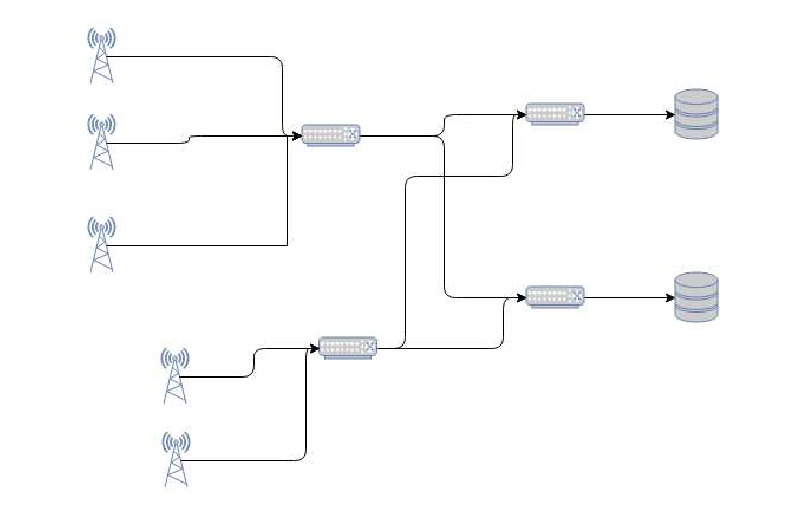
\includegraphics[scale=0.5]{fronthaul}



	 \end{minipage} 
 \hfill
 \begin{minipage}[c]{.45\linewidth}
	
	
	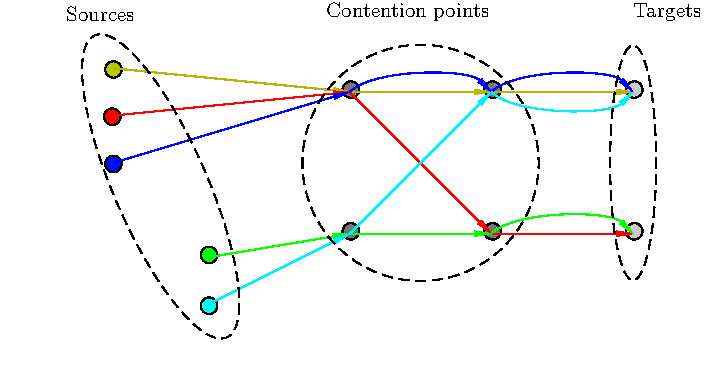
\includegraphics[scale=0.5]{graphmodel}\\

	 \end{minipage}
	 
\caption{A C-RAN fronthaul network and its corresponding routed network}
\label{fig:fronthaul}
\end{figure} 

	The  \textbf{contention depth} of a routed network $(G,{\cal R})$ is equal to the maximum of the contention level over all vertices. It is the number of contention points on the longest route of the network. In all the article, $(G,{\cal R})$ is the routed network, ${\cal C}$ is the set of its contention vertices, $n$ denotes $|\cal{R}|$ the number of routes.  

  %\subsection{Network modeling}
  
%The network is modeled as a directed graph $G=(V,A)$. Each arc  $(u,v)$ in $A$ is labeled by an integer weight $\Omega(u,v)$ which represents the time taken by a message to go from $u$ to $v$ using this arc. A {\bf route} $r$ in $G$ is a directed path, that is, a sequence of adjacent vertices $u_0, \ldots , u_{l}$, with $(u_i,u_{i+1}) \in A$.  The {\bf latency} of a vertex $u_i$ in a path $r=(u_0,\dots,u_l)$ is defined by $\lambda(u_i,r)= \sum\limits_{0 \leq j <i} \Omega(u_j, u_{j+1})$. We also define $\lambda(u_0,r)=0$. The length of the route $r$ is defined by $\lambda (r)= \lambda (u_l,r)$.
%We denote by $\cal R$ a set of routes, the pair $(G,\cal R)$ is called a {\bf routed network} and represents our telecommunication network.
%The first vertex of a route models an antenna (RRH) and the last one a data-center (BBU) which processes the messages sent by the antenna.

   %\subsection{Messages dynamic}
	 
    %Time is discretized, hence the unit of all time values is a slot, the time needed to transmit a minimal unit of data over the network. The weight of an arc is also expressed in slots, it is the time needed by a message to go through this arc.
     %   In the process we study, a message is sent on each route at each period, denoted by $P$.
      %Let $r=(u_0,\dots,u_l)$ be a route, if a message is sent at time $m$ from $u_0$ the first vertex of $r$ then it will arrive at vertex $u_i$ in $r$ at time $m + \lambda(u_i,r)$. Since the process is periodic, if the message from $r$ goes through an arc at time $t\in [0,P-1]$, 
      %then it goes through the same arc at time $t+kP$ for all positive integers $k$. Therefore, every time value can be computed modulo $P$ and we say that the first time slot at which a message sent at time $m$ on $r$ reaches a vertex $u_i$ in $r$ is $t(u_i,r) = m + \lambda(u_i,r)\mod P$. 
      
      %A message usually cannot be transported in a single time slot. We denote by $\tau$ the number 
      %of \emph{consecutive slots} necessary to transmit a message. In this paper, we assume that $\tau$ is the same for all routes. Indeed, the data flow sent by an RRH to its BBU is the same, regardless of the route. Let us call $[t(u,r)]_{P,\tau}$ the set of time slots used by route $r$ at vertex $u$ in a period $P$, that is $[t(u,r)]_{P,\tau} = \{t(u,r) + i \mod P \mid 0 \leq i < \tau \}$. 
%       Usually $P$ and $\tau$ will be clear from the context and we will denote $[t(v,r)]_{P,\tau}$ by $[t(v,r)]$.
      %Let $r_1$ and $r_2$ be two routes, on which messages are sent at time $m_1$ and $m_2$ in their first vertex.
      %We say that the two routes have a {\bf collision} if they share an arc $(u,v)$ and $[t(u,r_{1})]_{P,\tau} \cap [t(u,r_{2})]_{P,\tau} \neq \emptyset$.
      
       %  A {\bf $(P,\tau)$-periodic assignment} of a routed network $(G,\cal R)$ is a function that associates to each route 
        % $r \in \cal R$ its \textbf{offset} $m_r$ that is the time at which a message is emitted at the first vertex of the route $r$.  In a $(P,\tau)$-periodic assignment, \emph{no pair of routes has a collision}.
	 
	 
 \subsection{Dynamic of Datagrams Transmissions}
	    
 		In this article, we consider a discretized time. The unit of time is called a {\bf tic}. This is the time needed to send an atomic data in a link of the network. We assume that the speed of the links is the same over all the network. Several of the authors are developing a prototype based on ethernet base-X~\cite{ieee_8023}, using standard values for the parameters of the network: the size of an atomic data is $64$ bits, the speed of the links is $10$Gbps, and the length of a tic is thus about $6.4$ nanoseconds. 

        In the process we study, a message called a {\bf datagram} is sent on each route from the source node. The \textbf{size} of a datagram is an integer, denoted by $\tau$, it is the number of tics needed by a node to emit the full datagram through a link.  In this paper, we assume that $\tau$ is the same for all routes. It is justified by our application to C-RAN, where all source nodes are RRHs sending the same type of message. There is no preemption: Once a datagram has been emitted, it cannot be fragmented during its travel in the network. 


        \textbf{TODO:} on propose de faire du buffering que dans les BBUs qui correspondent à un troisième ensemble de sommets dans le modèle. On explique les offsets. Un assignement, c'est la donnée
        de $((o_i,w_i))$. Dire qu'on peut faire des modèles avec attente dans chaque noeud.
In this article, we strongly restrict where buffering can take place. We only allow a positive buffering to take place in the BBU, hence for each route 
        $r$, there is a single contention point $u$ such that $A(r,u)$ can be larger than zero and we call
        this value the waiting time of $r$, denoted by $w_r$. 

        The arrival of datagram in antennas need no to be synchronized, and we can decide when in the period
        each datagram is available in the first vertex of its route. If  





          Let $r=(u_0,\dots,u_l)$ be a route. In order to avoid contention, it is possible to buffer datagrams in contention points. The function $A$, called an \textbf{assignment}, associates an integer value, greater or equal to $0$, to each couple (route,vertex) of the routed network $(G,{\cal R})$. Those integers represent the buffering time of the datagrams in the nodes of the network: a datagram of route $r$ waits $A(r,u)$ tics in the buffer of vertex $u$. 
          Let $u$ be the first vertex of the route $r$, we say that $A(r,u)$ is the offset of the 
          route $r$.         
       

 The \textbf{arrival time} of a datagram in vertex $u_i$ of $r$, is the first time at which the datagram sent on $r$ reaches $u_i$, and is defined by $t(r,u_i) = \lambda(u_i,r) + \sum_{k=0}^{i-1} A(r,u_k) $. The date at which a datagram reaches a vertex $u_i$ is decomposed into a \emph{physical delay} due to the time to go through the links before $u_i$ and a \emph{logical} delay caused by the use of buffers as determined by assignment $A$.

 
%   In the application we study the full transmission time is bounded . We define $Tmax$ such that $TR(A) \leq Tmax$.
     
 \subsection{Periodic Emission of Datagrams}

 	The process we model in this article is \emph{periodic}: for each period of $P$ tics, a datagram is ready to be sent from each source node in the network at time zero of the period. The process is assumed to be infinite, since it should work for an arbitrary number of periods. We chose to always use the same waiting time in all periods, for simplicity of implementation in real networks but also to make our problem more tractable from a theoritical perspective. In other words, at the same time of two different periods, all messages are at the same position in the network: the assignments we build are themselves periodic of period $P$. Thus, we only need to consider the behavior of the datagrams on each node of the network during a single period, and to apply the same pattern to every subsequent period. 
    Let us call $[r,u]_{P,\tau}$ the set of tics used by a datagram on $r$ at vertex $u$ in a period $P$, that is $[r,u]_{P,\tau} = \{t(r,u) + i \mod P \mid 0 \leq i < \tau \}$. 

      Let us consider two routes $r_1$ and $r_2$, they have a {\bf collision} at the contention point $u$ if and only if $[r_1,u]_{P,\tau} \cap [r_2,u]_{P,\tau} \neq \emptyset$.\\

        An assignment $A$ of a routed network $(G,{\cal R})$ is said to be \textbf{valid} if \emph{no pair of routes has a collision}. 
        The validity of an assignment depends on $P$ the period and $\tau$ the size of the messages,
        thus we say that $A$ is a valid $(P,\tau)$ assignment. When $P$ and $\tau$ are fixed or clear from the context, we say that $A$ is a valid assignment.
        Note that the period $P$, as well as the size of a message $\tau$ is fixed in our $C-RAN$ application, but not the buffering policy. 
         Hence, the aim of our work is to find a valid assignment which minimizes the latency of transmissions over the network, that is $TR(A)$.
       \\ 

  If $u_l$ is the last vertex of the route $r$, the transmission time of the datagram on 
  $r$ is denoted by $TR(A,r)$ and is equal to $t(r,u_l)$. We define the \textbf{transmission time} of an assignment $A$ as $TR(A) = \displaystyle \max\limits_{r \in {\cal R}} TR(A,r) $. This is the time elapsed before the reception of the beginning of the last datagram. 
       
       \noindent {\bf Periodic Assignment for Low Latency (\pall)} 

      \noindent {\bf Input:}  Routed network $(G,{\cal R})$, period $P$, datagram size $\tau$.%, a bound on the latency $T$.
      
      %\noindent {\bf Decision problem:} is there a valid assignment $A$ of $(G,{\cal R})$ such that $ TR(A) \leq T$ ?

      \noindent {\bf Output:} assignment $A$ which minimizes $TR(A)$.
      \\






      As an example of a $(2,1)$-periodic assignment, let us consider a routed network 
      where all pairs of routes intersect at a different arc. It is easy to design such a network and an example is given in Figure~\ref{fig:example}. We set $\tau = 1$ and the weights are chosen so that if $r_{i}$ and $r_{j}$ have $u$ as first common vertex then we have $\lambda(u,r_{i}) - \lambda(u,r_{j})=1$. There is a $(2,1)$-periodic assignment by setting all $m_{i}$ to $0$.

  
      \begin{figure}[ht]
      \begin{center}
          \scalebox{0.47}{
          
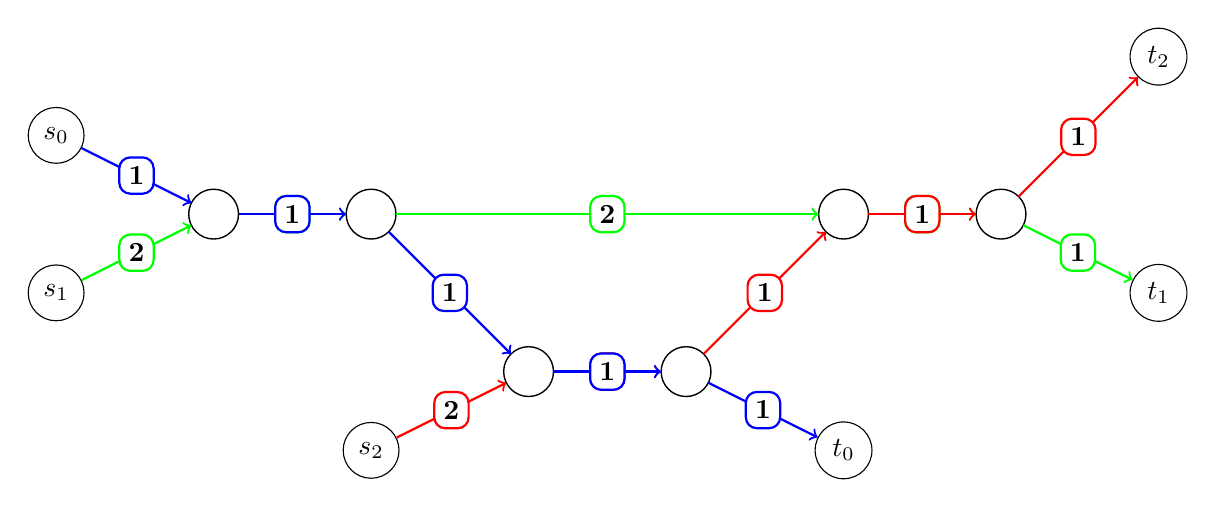
\begin{tikzpicture}


\tikzset{
  LabelStyle/.style = { rectangle, rounded corners, draw,
                       font = \bfseries },
  EdgeStyle/.append style = {->} }
  \SetGraphUnit{5}
  \node[draw,circle] (s3) at (4, 2) {$s_2$}; 
  \node[draw,circle] (s2) at (0, 4) {$s_1$}; 
  \node[draw,circle] (s1) at (0, 6) {$s_0$}; 

  \node[draw,circle] (t3) at (14, 7) {$t_2$}; 
  \node[draw,circle] (t2) at (14, 4) {$t_1$}; 
  \node[draw,circle] (t1) at (10, 2) {$t_0$}; 

  
  \SetVertexNoLabel
  \Vertex[x=2,y=5]{A}
  \Vertex[x=4,y=5]{B}
  \Vertex[x=10,y=5]{C}
  \Vertex[x=12,y=5]{D}
  \Vertex[x=6,y=3]{E}
  \Vertex[x=8,y=3]{F}
  \tikzset{
  EdgeStyle/.append style = {green} }
  \Edge[label = 2](s2)(A)
  \Edge[label = 1](A)(B)
  \Edge[label = 2](B)(C)
  \Edge[label = 1](C)(D)
  \Edge[label = 1](D)(t2)

  
   \tikzset{
  EdgeStyle/.append style = {red} }
  \Edge[label = 2](s3)(E)
  \Edge[label = 1](E)(F)
  \Edge[label = 1](F)(C)
  \Edge[label = 1](C)(D)
  \Edge[label = 1](D)(t3) 
     \tikzset{
  EdgeStyle/.append style = {blue} }
  \Edge[label = 1](s1)(A)
  \Edge[label = 1](A)(B)
  \Edge[label = 1](B)(E)
  \Edge[label = 1](E)(F)
  \Edge[label = 1](F)(t1)

\end{tikzpicture}

}
     \end{center}
       \caption{A routed network with $(0,0,0)$ as a $(2,1)$-periodic assignment}
       \label{fig:example}
      \end{figure}

      \subsection{Periodic route assignment}\label{nonmonotone}

    We want to find an assignment which allows to send periodic messages from sources to targets
    without collisions. We introduce the following associated decision problem, useful for hardness proofs.
    

      \noindent {\bf  Periodic Routes Assignment (\pra)} 

      \noindent {\bf Input:} a routed network $(G,\cal R)$, an integer $\tau$ and an integer $P$.

      \noindent {\bf Question:} does there exist a $(P,\tau)$-periodic assignment of $(G,\cal R)$ ?


      We will prove in Section~\ref{sec:complexity} that the problem \pra is $\NP$-complete, even in restricted settings.
      In fact, approximating the smallest value of $P$ for which there is a $(P,\tau)$-periodic assignment is already hard.
      
      An unusual property of assignment is that given a routed network, we may have a $(P,\tau)$-periodic assignment but no
      $(P',\tau)$-periodic assignment with $P' > P$: the existence of an assignment is not monotone with regard to $P$.

	\begin{lemma} \label{lemma:monotonic}
	 For any odd $P$, there is a routed network such that there is a $(2,1)$-periodic assignment but no $(P,1)$-periodic assignment.
	\end{lemma}
\begin{proof}

      We consider a generalization of the routed network $(G,{\cal R})$ given in Figure~\ref{fig:example}. 
      There are $n$ routes in the routed network and each pair of routes $(r_i,r_j)$ share a single arc, which is not in any other route. The weights are chosen so that for $v$, the first vertex which belongs to $r_i$ and $r_j$, we have $\lambda(v,r_i) - \lambda(v,r_j)= P$, where $P$ is an odd number smaller than $n$. In such a graph, there is no $(P,\tau)$-periodic assignment, since the problem reduces to finding a $P$-coloring in a complete graph with $n > P$ vertices, the colors being the offsets of the routes.\\
      If we consider a period of $2$, for all $i \neq j$, $\lambda(v,r_i) - \lambda(v,r_j) \mod 2 = 1$ . Therefore $(0,\dots,0)$ is a $(2,1)$-periodic assignment of ${\cal R}$.      
\end{proof}
      
      
      \subsection{Periodic assignment for low latency}
      
   In the context of cloud-RAN applications, we need to send a message from an RRH $u$ to a BBU $v$ and then 
      we must send the answer from $v$ back to $u$. We say that a routed network $(G, {\cal R})$ is \textbf{symmetric} if the set of routes is partitioned into the sets $F$ of \textbf{forward routes} and $B$ of \textbf{backward routes}. There is a bijection $\rho$ between $F$ and $B$ such that for any forward route $r \in F$ with first vertex $u$ and last vertex $v$, the backward route $\rho(r) \in B$ has first vertex $v$ and last vertex $u$. In all practical cases the routes $r$ and $\rho(r)$ will be the same with the orientation of the arcs reversed, which corresponds to bidirectional links in \emph{full-duplex} networks, but we need not to enforce this property.
         
      We now give a new interpretation of a $(P,\tau)$-periodic assignment of a $(G,{\cal R})$ symmetric routed network, so that it represents the sending of a message and of its answer.
      This assignment represents the following process: First a message is sent at $u$, through the route $r \in F$, at time $m_r$.
      This message is received by $v$, i.e., the last vertex of $r$ at time $t(v,r)$. The answer is then sent back to $u$ on the route $\rho(r)$ in the same period at time $m_{\rho(r)}$ if $m_{\rho(r)} > t(v,r)$, otherwise at time $m_{\rho(r)}$ in the next period. The time between the arrival of the message and the time it is sent back is called the \textbf{waiting time} and is defined by $w_r = m_{\rho(r)} - t(v,r)$ if $m_{\rho(r)} > t(v,r)$ and $w_r = m_{\rho(r)} + P - t(v,r)$ otherwise. Figure~\ref{fig:assignment} illustrates this process in an RRH and its corresponding BBU.
 
     \begin{figure}[h]
      \begin{center}
      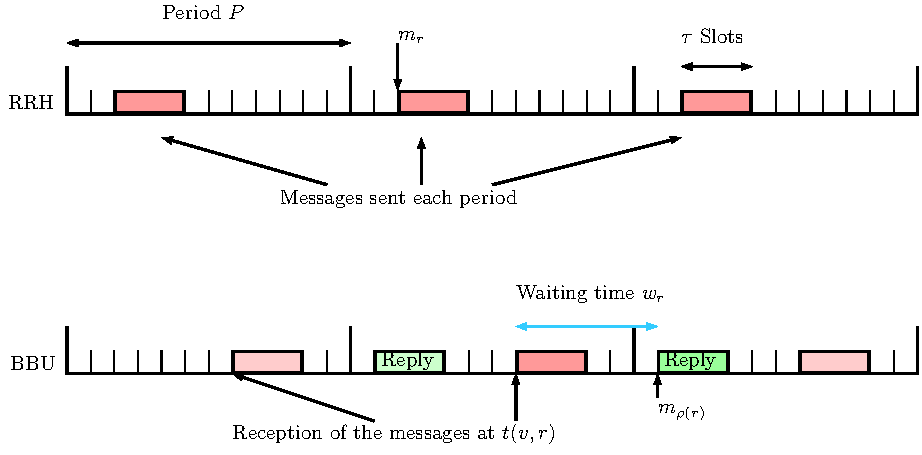
\includegraphics[width=0.47\textwidth]{rrh.pdf}
      \end{center}
      \caption{Periodic process}\label{fig:assignment}
      \end{figure}
      
      Note that, in the process we describe, we do not take into account the computation time a BBU needs to deal with one message. It can be encoded in the weight of the last arc leading to the BBU and thus we do not need to consider it explicitly in our model. 
      The whole process time for a message sent on the route $r$ is equal to $PT(r)=\lambda(r)+ w_r+\lambda(r)$.      
      In the process time, we count the time between the time the first slot of the message is emitted and the first time at which the first slot of the message comes back. Alternatively we could consider the time between the emission of the first slot and the reception of the last slot of the message, which adds $\tau$ to the process time. Both definitions are equivalent in our context where all messages are of size $\tau$, hence we chose the first definition which is slightly simpler. 
      Each route must respect a time limit that we call \emph{deadline}. To represent these deadlines, 
      we use a deadline function $d$, which maps to each route $r$ an integer such that $PT(r)$ must be less than $d(r)$.
      
%     The {\bf maximum process time} of the assignment $m$ of $(G,{\cal R})$ is defined by $MPT(m)=\max\limits_{r \in {\cal R}} PT(r)$.
      We consider the following decision problem.

      \noindent {\bf Periodic Assignment for Low Latency (\pall)} 

      \noindent {\bf Input:}  A symmetric routed network $(G,{\cal R})$, the integers $P$, $\tau$ and a deadline function $d$.
      
      \noindent {\bf Question:} does there exist a $(P,\tau)$-periodic assignment $m$ of $(G,{\cal R})$ such that for all $r \in {\cal R}$, $PT(r) \leq d(r)$?

      As a consequence of the $\NP$-hardness of \pra, we show in the next subsection that this problem is $\NP$-hard. 
      In Section~\ref{sec:PALL} we will study heuristics used to solve the search version of \pall (computing an assignment), also denoted by \pall for simplicity. In \pall, we have chosen to bound the process time of each route, in particular we can control the worst case latency. It is justified by our C-RAN application with hard constraint on the latency. It would be interesting to study the case of a constraint on the \emph{average} of process times (or equivalently waiting times) of routes, which may be more relevant in other contexts.

     
      The following table summarize the main notations used in the paper.
      \begin{center}
   \begin{tabularx}{0.5\textwidth}{|c|X|}
    \hline
     $(G,\cal R)$ & Routed network \\
     \hline
      $\Omega(u,v)$ & Weight of the arc $(u,v) \in A$ \\
      \hline
      $\lambda(u_i,r)$ & Latency of the vertex $u_i$ in $r$\\
         \hline
         $\lambda(r)$ & Length of the route $r$\\
         \hline
         $P$ & Period\\
         \hline
         $\tau$ & Size of a message\\
         \hline
         $ [t(v,r)]$& Set of time slots used by route $r$ at vertex $v$ in a period $P$\\
         \hline 
         $m=(m_0, \ldots ,m_{n-1})$& Assignment: an offset for each route\\
              \hline 
         $w_r$& Waiting time of the route $r$\\
            \hline 
         $PT(r)$& Process time of the route $r$\\
           \hline 
       $d(r)$ & Deadline of the route $r$\\
    \hline

      \end{tabularx}
      \end{center}


\section{Hardness of \pra}
  \label{sec:complexity}

 In this section we always assume that the size of a message $\tau$ is equal to one. 
 We will prove the hardness of \pra and \pall for $\tau =1$ which implies the hardness of problems with $\tau$ unconstrained. 
Consider an instance of the problem \pra, i.e., a routed network $(G,\cal{R})$ and a period $P$.
The {\bf conflict depth} of a route is the number of arcs of the route which also belong to other routes.
The conflict depth of a routed network $(G,\cal{R})$ is the maximum of the conflict depth of its routes.
The {\bf conflict width} of a routed network is the maximal number of routes sharing the same arc.
Remark that a $(P,1)$-periodic assignment must satisfy that $P$ is larger or equal to its conflict width.


We give two alternate proofs that \pra is $\NP$-complete.
The first proof works already for conflict depth two. Remark that for conflict depth one,
the graph can be seen as a set of disjoint pair of routes, on which \pra and \pall can be solved in linear time. 
 The second proof reduces the problem to graph coloring and implies inapproximability when one tries to find the smallest possible $P$.  Finally, it is easy to see that \pra is easy on trees and it may be interesting to study its complexity on 
 bounded treewidth networks, since it is a common property of real networks~\cite{de2011treewidth}.
 

 \begin{theorem}
Problem \pra is $\NP$-complete on the class of routed networks with conflict depth two.
\end{theorem}
 \begin{proof}
 Problem \pra is in $\NP$ since given an offset for each route in an assignment, it is easy to check in linear time with regard to the number of arcs whether there are collisions.
 
  Let $H=(V,E)$ be an undirected graph and let $d$ be its maximal degree. We consider the problem to determine whether $H$ is arc-colorable  with $d$ or $d+1$ colors. The arc coloring problem is $\NP$-hard~\cite{holyer1981np} and we reduce it to \pra to prove its $\NP$-hardness. To do that, we define from $H$ a routed network $(G,{\cal R})$ as follows.
  The vertices of $G$ are $v_1, v_2$ for each $v$ in $V$ and $s_{u,v}, t_{u,v}$ for each $(u,v) \in E$.
  For each arc $(u,v) \in E$, there is a route $s_{u,v},u_1,u_2,v_1,v_2,t_{u,v}$ in ${\cal R}$. 
  
   To define ${\cal R}$ an arbitrary orientation of each edge is chosen. 
   Then for each arc $(u,v)$ there is a route $s_{u,v},u_1,u_2,v_1,v_2,t_{u,v}$ in ${\cal R}$.
  All these arcs are of weight $0$. The set of arcs of G is the union between all the arcs of the previously defined routes.
   
  Observe that the existence of a $d$-coloring of $H$ is equivalent to the existence of a $(d,1)$-periodic assignment
  of $(G,{\cal R})$. Indeed, a $d$-coloring of $H$ can be seen as a labeling of its arcs by the integers
  in $[d]$ and we have a bijection between $d$-colorings of $H$ and offsets of the routes of ${\cal R}$.
  By construction, the constraint of having no collisions between the routes is equivalent to the fact that no two adjacent arcs have the same color. Therefore we have reduced arc coloring to \pra by a polynomial time transformation which concludes the proof. 
 \end{proof}
 
 Remark that we have used zero weights in the proof. If we ask the weights to be strictly positive, which makes sense in our model since they represent the delay of physical links, it is easy to adapt the proof. We just have to set them so that in any route the weight at $u_1$ is equal to $d$ and thus equal to $0$ modulo $d$. We now lift this hardness result to the problem \pall.

\begin{corollary}
Problem \pall is $\NP$-complete on the class of routed networks of conflict depth two.
\end{corollary}
\begin{proof}
 We consider $((G,{\cal R}),P,\tau)$ an instance of \pra. We assume that no vertex is the first of some route and the last of another one. Remark that this condition is satisfied in the previous proof, which makes the problem \pra restricted to this kind of instance $\NP$-complete. 
 Let us define $d(r) = 2 \times \max_{r' \in {\cal R}} \lambda(r') + P$. We define $(G',{\cal R}')$ a symmetric routed network from $(G,{\cal R})$ where for every route we add a symmetric route with new arcs of opposite orientation and the same weights.
 We prove that the instance $((G',{\cal R'}),P,\tau,d)$ is in \pall if and only if $((G,{\cal R}),P,\tau)$ is in \pra.
 If $((G',{\cal R'}),P,\tau,d)$ is in \pall, then a $(P,\tau)$-assignment of $(G',{\cal R'})$ restricted to $\R$ is a $(P,\tau)$-assignment of $((G,{\cal R})$ since they cannot be any collision between routes of ${\cal R}$.
 
 Assume now that $((G,{\cal R}),P,\tau)$ is in \pra. First, remark that the waiting time of each route is by definition less than $P$ and thus we have for all $r\in {\cal R}$, $PT(r) \leq d(r)$. Moreover a $(P,\tau)$-assignment of $(G,{\cal R})$ can be extended into a $(P,\tau)$-assignment of $(G',{\cal R'})$ in the following way. For each route $r \in \cal{R}$ of last vertex $v$, the time at which the message arrives is $t(v,r)$, then we choose as offset for $\rho(r) \in \cal{R}'$ $-t(v,r) \mod P$. The symmetry ensures that each new route $\rho(r)$ in ${\cal R'}$ uses exactly the same time slots as $r$ on each of its node and thus avoid collisions.
\end{proof}

Let \minpra be the problem, given a routed network and an assignment, to find the minimal period $P$ such that there is a $P$-periodic assignment. 

\begin{theorem}\label{th:inapprox}
If $\P \neq \NP$, problem \minpra on the classes of routed networks of conflict width two cannot be approximated in polynomial time within a factor $n^{1-o(1)}$ where $n$ is the number of routes.
\end{theorem}

\begin{proof}
 We reduce graph coloring to \pra. Let $H$ be a graph instance of the $k$-coloring problem. 
 We define ${\cal R}$ in the following way: for each vertex $v$ in $H$, there is a route $r_v$ in ${\cal R}$.
 Two routes $r_v$ and $r_u$ share an arc if and only if $(u,v)$ is an arc in $H$; this arc is the only one shared by these two routes. All arcs are of weight $0$. Note that it is easy to build a graph with such routes as in Figure~\ref{fig:reduction}.
 
 Observe that the existence of a $k$-coloring of $H$ is equivalent to the existence of a $(k,1)$-periodic assignment in $G$, 
 by converting an offset of a route into a color of a vertex and reciprocally. Therefore if we can approximate the minimum value of $P$ within some factor, we could approximate the minimal number of colors needed to color a graph within the same factor. The proof follows from the hardness of approximability of finding a minimal coloring~\cite{zuckerman2006linear}.
\end{proof}


In particular, this reduction shows that even with small maximal load, the minimal period can be large.

    \begin{figure}[ht]
    \centering
    \scalebox{0.37}{
    \begin{tikzpicture}
    \tikzset{
      LabelStyle/.style = { rectangle, rounded corners, draw,
			  font = \bfseries },
      EdgeStyle/.append style = {->} }
      \SetGraphUnit{5}
      
      
      \node[draw,circle] (s3) at (4, 2) {$s_2$}; 
      \node[draw,circle] (s2) at (0, 4) {$s_1$}; 
      \node[draw,circle] (s1) at (0, 6) {$s_0$}; 

      \node[draw,circle] (t3) at (12, 3) {$t_2$}; 
      \node[draw,circle] (t2) at (14, 4) {$t_1$}; 
      \node[draw,circle] (t1) at (10, 2) {$t_0$}; 
      

      \tikzstyle{VertexStyle}=[shape = circle, draw, minimum size = 20pt]
	\tikzset{
      VertexStyle/.append style = {blue} }
	\Vertex[x=-8,y=3]{1}
	      \tikzset{
      VertexStyle/.append style = {green} }
	  \Vertex[x=-7,y=5]{2}

	    \tikzset{
      VertexStyle/.append style = {red} }
	  \Vertex[x=-6,y=4]{3}
		\tikzset{
      VertexStyle/.append style = {black} }
      
      
      \SetVertexNoLabel
      \Vertex[x=2,y=5]{A}
      \Vertex[x=4,y=5]{B}
      \Vertex[x=10,y=5]{C}
      \Vertex[x=12,y=5]{D}
      \Vertex[x=6,y=3]{E}
      \Vertex[x=8,y=3]{F}
      \tikzset{
      EdgeStyle/.append style = {green} }
      \Edge(s2)(A)
      \Edge ([yshift=-0.5ex]A.east)([yshift=-0.5ex]B.west)
      \Edge(B)(C)
      \Edge(C)(D)
      \Edge(D)(t2)

      
      \tikzset{
      EdgeStyle/.append style = {red} }
       \Edge ([yshift=-0.5ex]E.east)([yshift=-0.5ex]F.west)
      \Edge(s3)(E)
      \Edge(F)(t3) 
	\tikzset{
      EdgeStyle/.append style = {blue} }
      \Edge(s1)(A)
     \Edge ([yshift=0.5ex]A.east)([yshift=0.5ex]B.west)
      \Edge(B)(E)
             \Edge ([yshift=0.5ex]E.east)([yshift=0.5ex]F.west)
      \Edge(F)(t1)
      
	\tikzset{
      EdgeStyle/.append style = {black,-} }

      \Edge(1)(2)
      \Edge(1)(3)
    \node (1) at (-3,4){\Huge $\rightarrow$};
%     
%     \node (2) at (-7,0){\Huge H};
%     \node (3) at (10,0){\Huge G};
    \end{tikzpicture}
    }
    \caption{Reduction from k-coloring to \minpra}
    \label{fig:reduction}
    \end{figure}
    
\section{The Star Routed Network} \label{sec:star_routed_network}
  
   
    
       Let us define a family of simple routed networks modeling a Point-to-Multipoint fronthaul (PtMP), which has been designed for C-RAN \cite{tayq2017real}. 
      The graph $G$ has two sets of vertices, $S=\{s_0,...,s_{n-1}\}$ and $T=\{t_0,...,t_{n-1}\}$ of cardinality $n$ and two special nodes: the central source node {\bf $c_s$} and the central target node {\bf $c_t$}.
      There is an arc between {\bf $c_s$} and {\bf $c_t$} and for all $i$, there is an arc between $s_i$ and $c_s$ and between $t_i$ and $c_t$. All the symmetric arcs are also in the graph with the same weights.
      The forward routes are the directed paths $r_i = (s_i,c_s,c_t,t_i)$ and $\rho(r_i) = (t_i,c_t,c_s,s_i)$ which define a symmetric routed network. 
      The symmetric routed networks $(G, \{r_i,\rho(r_i)\}_{i<n})$ is called a \textbf{star routed network}. This topology may seem simplistic, but every network in which all routes share an arc can be reduced to a star routed network. It is common in fronthaul networks, since often all the BBUs are located in the same data-center. In such a situation, we can see the weights of the arcs $(c_t,t_i)$ either as all equals (in that case, the problem is trivial, see Section \ref{sec:PALL}) or different due to the structure of the network inside the data-center and the various hardwares used for different BBUs. This topology has conflict depth one (but a maximal conflict width), hence \pra can be solved in polynomial time.
      \begin{figure}
       \begin{center}
	 \scalebox{0.8}{
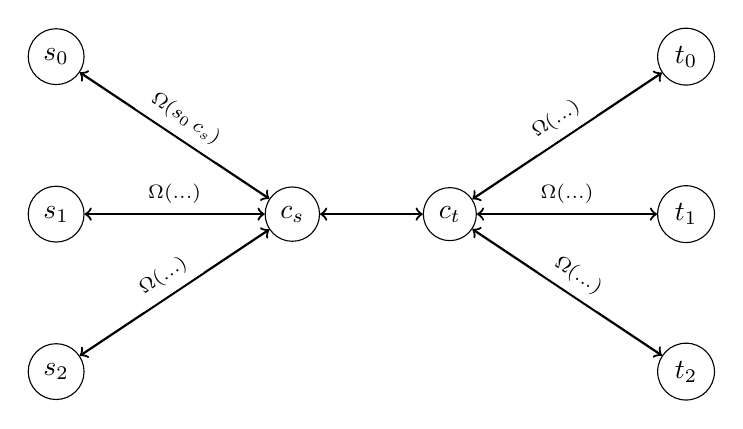
\begin{tikzpicture}

\tikzset{EdgeStyle/.style={<->,font=\scriptsize,above,sloped,midway}}
  \SetGraphUnit{5}
  
  \node[draw,circle] (s3) at (0, 0) {$s_2$}; 
  \node[draw,circle] (s2) at (0, 2) {$s_1$}; 
  \node[draw,circle] (s1) at (0, 4) {$s_0$}; 

  \node[draw,circle] (t3) at (8, 0) {$t_2$}; 
  \node[draw,circle] (t2) at (8, 2) {$t_1$}; 
  \node[draw,circle] (t1) at (8, 4) {$t_0$}; 
  

  \node[draw,circle] (cs) at (3, 2) {$c_s$}; 
  \node[draw,circle] (ct) at (5, 2) {$c_t$}; 

  
  \Edge[label = $\Omega(s_0\,c_s)$](s1)(cs)
  \Edge[label = $\Omega(...)$](s2)(cs)
  \Edge[label = $\Omega(...)$](s3)(cs)
  
  \Edge[label = $\Omega(...)$](ct)(t1)
  \Edge[label = $\Omega(...)$](ct)(t2)
  \Edge[label = $\Omega(...)$](ct)(t3)
  
  \Edge(cs)(ct)

  
\end{tikzpicture}
}

  \end{center}
  \caption{A star routed network}
  \end{figure}
	
	
  When solving $\pall$ on a star routed network, we can do several assumptions on the parameters of the network  without loss of generality. 
  
  \begin{proposition}\label{prop:canonical}
   Let $I = ((G,{\cal R}), P, \tau , d)$ be an instance of \pall, then there is another instance 
   $I' = ((G',{\cal R}), P, \tau , d')$ such that:
   \begin{itemize}
    \item $I \in \pall \Leftrightarrow I' \in \pall$
    \item $\Omega(c_s,c_t) = 0$
    \item $\forall i<n, \, \Omega(s_i,c_s) =0$
    \item $\forall i<n, \, \Omega(c_t,t_i) + \Omega(t_i, c_t) < P$
   \end{itemize}
  \end{proposition}

  \begin{proof}
   We explain how we build $G'$ and $d'$ from $G$ and $d$ in such a way that there is a bijection 
   between the satisfying assignments of $I$ and $I'$, which proves the proposition.
    
  The central arc appears in every route, therefore when we change it, it does not change 
  the satisfying assignments. If we subtract twice its weight to $d(r)$ for each $r$, and set its
  weight to zero in $G'$, then the constraints $PT(r) \leq d(r)$ will be the same in $I$ and $I'$.
      
  In $G'$, the weights of the arcs $(s_i,c_s)$ is set to $0$ and $2\Omega(s_i,c_s)$
  is subtracted to $d(r_i)$. Hence the deadline constraints are the same in $I$ and $I'$.
  There is a bijection between the assignments of $I$ and $I'$ by mapping $m_i$ to $m_i + \Omega(s_i,c_s)$.
  
  Finally, we can subtract $P/2$ to $\Omega(c_t,t_i)$ and $\Omega(t_i,c_t)$ if we subtract $P$ to $d(r_i)$.
  The constraints on collisions of message are modulo $P$ and thus do not change. The deadline constraints are left unchanged since the two modifications cancel out. Therefore to obtain $I'$, we remove $P/2$ enough time to each  $\Omega(t_i,c_t)$ and $\Omega(c_t,t_i)$ so that $\Omega(c_t,t_i) + \Omega(c_t,t_i)< P$. 
  \end{proof}

   From now on, we assume that all star routed networks have the properties given in Proposition~\ref{prop:canonical}.
  Collisions between messages can only appear on the arc $(c_s,c_t)$ between forward routes or on the arc $(c_t,c_s)$
  between backward routes. The flow of messages in a star routed network is completely described by their repartition in two time windows of size $P$, the {\bf forward period} which contains all $[t(c_s,r)]_{P,\tau}$ with $r$ a forward route and the {\bf backward period} which contains all $[t(c_t,r)]_{P,\tau}$ with $r$ a backward route.

\section{Assignments with no waiting time} \label{sec:PAZL}
  
  In this subsection, we deal with a simpler version of the problem \pall.
  We ask for a $(P,\tau)$-periodic assignment {\bf with all waiting times equal to $0$}, that is $d(r) = 2\lambda(r)$ and we call this restriction {\bf Periodic Assignment for Zero Latency} or \pazl. We study \pazl since it is simpler, in particular 
  choosing the offset $m_r$ also sets the offset of the route $\rho(r)$ to $m_{\rho(r)} = m_{r} + \lambda(r) \mod P$.
  We get better theoretical results and practical algorithms for \pazl than for \pall. Moreover, as we show in our experimentations of Section~\ref{sec:exp_PAZL}, this problem can very often be solved positively (albeit less often than the general problem). Finally, a solution to \pazl is simpler to implement in real telecommunication networks, since we do not need to implement any buffering at all.    
  
   The problem \pazl is similar to the minimization of makespan in a two flow-shop with delays (see Section~\ref{sec:braheuristic}), a problem known to be $\NP$-complete~\cite{yu2004minimizing}. It suggests that \pazl is $\NP$-complete, however we have not been able to prove it yet,  because the periodicity is hard to deal with. With additional constraints we can get rid of the periodicity in the hardness proof, for instance if we consider that the central link is unidirectional, that is collisions can happen between messages going from $c_s$ to $c_t$ and messages  going from $c_t$ to $c_s$. This variant can be shown to be $\NP$-complete by a reduction from the subset sum problem as it is done for a similar problem of scheduling pair of tasks~\cite{orman1997complexity}.
  On the other hand we show positive results:  when the period is large or when the routes are short there is always a solution to \pazl and it can be found in polynomial time. We also give a fixed parameter tractable algorithm which finds a solution to \pazl if there is one in time exponential in the number of routes only. 
  
\subsection{Shortest-longest policy}
    

    We first present a simple policy, which works when the period is large with regard to the lengths of the routes.
    The messages are sent in order from the shortest route to the longest route, without any gap between two messages in the forward period.
    In other words, we assume that the route $r_i$ are sorted by increasing $\lambda(r_i)$ and we set $m_{r_i}$ the offset of $r_i$ to $i\tau$. We call this algorithm {\bf Shortest-Longest}.
      
     By definition, there are no collisions in the forward period and if the period is long enough, 
     it is easy to see that in the backward period the order of the messages are the same as in the forward period and that no collision can occur. 
      
      
      \begin{proposition} Let $(G, {\cal R})$ be a star routed network, and let $n\tau + 2(\lambda(r_{n-1}) - \lambda(r_{0})) \leq P$. There is a $(P,\tau)$-periodic assignment of $(G, {\cal R})$ with waiting times $0$ given by Shortest-Longest in time $O(n\log(n))$.\label{prop:SL}
      \end{proposition}
      \begin{proof}
       Since $m_{r_i} = i\tau$ and $n\tau < P$, $[t(c_s,r_{i})]_{P,\tau} = \{i\tau,\dots, (i+1)\tau -1\}$ and there are no collisions on the forward period.
       
       We may assume that $\lambda(r_{0}) = 0$, since removing $\lambda(r_{0})$ from every arc $(c_t,t_i)$ does not change the order on the length of the routes nor the collisions between messages.
       Since $\lambda(r_{0}) = 0$, by hypothesis we have $n\tau + 2\lambda(r_{n}) \leq P$ which implies that
       $[t(c_t,r_{i})]_{P,\tau} = \{2 \lambda(r_{i}) + i\tau, \dots,  2 \lambda(r_{i}) + (i+1)\tau -1\}$.
       Since $ \lambda(r_{i}) \leq  \lambda(r_{i+1})$ by construction, we have  $2 \lambda(r_{i}) + i\tau -1 < 2 \lambda(r_{i+1}) + (i+1)\tau$ which proves that there are no collisions on the backward period. 
 The complexity of the algorithm is dominated by the sorting of the routes in $O(n\log(n))$. 
      \end{proof}

      If the period is slightly smaller that the bound of Proposition~\ref{prop:SL}, a collision will occur on the first route in the backward period. Hence, this policy is not useful even as a heuristic for longer routes as confirmed by the experimental results of Subsection~\ref{sec:exp_PAZL}. 

   
    \subsection{Greedy algorithm}
    
    \textbf{TODO:} faire une preuve clean et montrer qu'on obtient des résultats assez bon,
    citer notre autre papier qui fait l'étude en détail. Ici, l'algo FPT est suffisant, car 
    on est sur des réseaux de 10/20 antennes.
    
      Let $\frac{n\tau}{P}$ be the \textbf{load} of a star routed network. The load is the proportion of time slots used by messages on the central arc in a period. Therefore if the load is larger than $1$ there cannot be an assignment. We propose a greedy algorithm to build a $(P,\tau)$-periodic assignment, which always finds an assignment when the load is less than $1/3$. Therefore in the rest of the article we will be only concerned with load larger than $1/3$.
    
    \begin{proposition}
    There is a $(P,\tau)$-periodic assignment of a star routed network with waiting times $0$ if the load is less than $1/3$ and it can be found in time $O(n^2)$.
    \end{proposition}
    \begin{proof}
     We consider the forward period and cut it into consecutive intervals of size $\tau$ that we call macro-slots. The algorithm works by choosing an offset for each route in the following way: try all offsets which put the message in a yet not used macro-slot in the forward
     period. Since the choice of an offset also sets the position of the message in the backward period, chose the first one which does not create a collision. We now prove that this algorithm always finds a $(P,\tau)$-periodic assignment without waiting time when $P \geq 3n\tau$ that is the load is less than $1/3$.
     
     Assume we are choosing the offset of the route $r_{k+1}$, we have at least $P - k \geq 3n - k$ free macro-slots in the forward period, since $P \geq 3n\tau$. Each of these $3n - k$ possible offset values translates into $3n - k$ positions of messages in the backward period. All these positions are separated by at least $\tau$ slots. There are already $k$ messages of size $\tau$ in the backward period. One such message can intersect at most $2$ potential positions since they are disjoint intervals. Therefore  amongst the possible $3n - k$ positions, there are  at least $3n - k -2k$ which are without collision. Since $k < n$, $3n - k -2k \geq 1$, which proves that the algorithm terminates and find a  $(P,\tau)$-periodic assignment. 
   
     This algorithm works with a complexity $O(n^2)$, since for the $k^{\text{th}}$ route we have to try at most $2k$ offsets before finding a correct one. We can test the $2k$ offsets of the backward period in time $O(k)$ by maintaining an ordered list of the intervals used by already set routes.
     \end{proof}
     \begin{figure}
      \begin{center}
      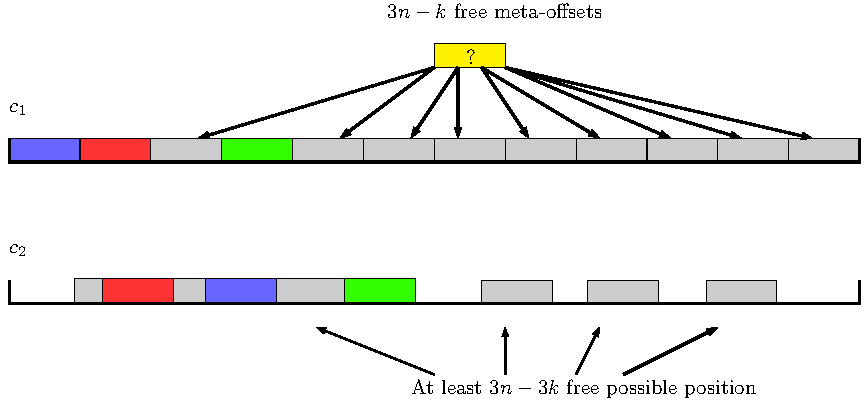
\includegraphics[width=0.48\textwidth]{ex3nt.pdf}
      \end{center}
      \caption{Forward and backward period, represented at step $k$ of the algorithm}
      \end{figure}
% 	\begin{algorithm}[H]
% 	\caption{Greedy assignment}
% 	\begin{algorithmic}
% 	\REQUIRE ${\cal R}_{\cal C}$, period $P$
% 	\ENSURE A P-periodic assignment in p $\leq P$, or FAILURE
% 	\STATE $T$ a table of the macro slots of size $\tau$ in the forward period.
% 	\STATE $L$ a list of free intervals in the backward period%$P2[P]$ slots backward period.
% 	\FORALL{source $s$ in S}
% 
% 	\FORALL{free intervals $[a,b]$ in $L$}
% 	\FORALL{ $a/\tau - \lambda(s) <j< b/\tau - \lambda(s)$ }
% 	\IF{ $T[j] == FREE$}
% 	\STATE $m_{s} \leftarrow j.\tau$
% 	\STATE $T[j] = USED$
% 	\STATE update $[a,b]$ in $L$
% 	\STATE BREAK
% 	\ENDIF
% 	\ENDFOR
% 	\ENDFOR
% % 	
% % 	\IF{No intervals are found for $s_i$}
% % 	\STATE return FAILURE
% % 	\ENDIF
% % 	\ENDFOR
% 
% 	\ENDFOR
% 
% 	\end{algorithmic}
% 	\end{algorithm}
	
This algorithm, contrarily to the previous one, may work well, even for loads higher than $1/3$.
In fact, experimental data in Subsection~\ref{sec:exp_PAZL} suggest that the algorithm finds a solution when the load is less than $1/2$. Note that we have experimented with other greedy algorithms which do not use macro-slots, they work even better in practice but they can be proved to work for load less than $1/4$ only.

\subsection{Compact assignment}

In this section we show how every assignment without waiting time can be put into a canonical form.
We use that to provide an algorithm which finds an assignment when it exists, in fixed parameter tractable time ($\FPT$) with parameter $n$ the number of routes (for more on parametrized complexity see~\cite{downey2012parameterized}). This is justified since $n$ is small in practice (from $10$ to $20$) and the other parameters such as $P$, $\tau$ or the weights are large.

Let $(G, {\cal R})$ be a star routed network and $m$ a $(P,\tau)$-periodic assignment.
A set of routes $S$ is \textbf{coherent} if for all $r \in {\cal R}$, $r \in S$ if and only if $\rho(r) \in S$. We say that a coherent set $S \subseteq {\cal R}$ is \textbf{compact} for the assignment $m$ if there is a route $r_0 \in S$ such that the following holds:  
for all coherent subsets $S'\subset S$ with $r_0 \notin S'$, if we remove $1$ from all offsets of routes in $S'$ then there is a collision with a route of $S \setminus S'$. We say that $m$ is compact if ${\cal R}$ is compact for $m$. 
% 
% 
% $r_1,r_2 \in {\cal R}$ two forward routes (resp. two backward routes) and 
%  We say that there is no gap between $r_1$ and $r_2$ in $\mathcal{M}$ if $\lambda(r_1,c_s) + \tau = \lambda(r_2,c_s)$ (resp. $\lambda(r_1,c_t) + \tau = \lambda(r_2,c_t)$). It means that the message of $r_2$ goes through the central arc just after the message of $r_1$ withtout wasting time. We say that a set of routes ${\cal R}$ is \textbf{compact} for the assignment $\mathcal{M}$ if for all forward routes $r \in {\cal R}$ but one, there is another forward route $r'$ such that there is no gap between $r'$ and $r$ or between $\rho(r')$ and  $\rho(r)$. If the set of all routes is compact for an assignment, we say that the assignment is compact.

\begin{proposition}
Let $(G, {\cal R})$ be a star routed network. If there is a $(P,\tau)$-periodic assignment of $(G, {\cal R})$, then there is a compact $(P,\tau)$-periodic assignment of $(G, {\cal R})$.
\end{proposition}
\begin{proof}
Consider $m$ a $(P,\tau)$-periodic assignment of $(G, {\cal R})$.
Let $r_0$ be an arbitrary route of ${\cal R}$,  and let $COMP = \{r_0\}$. Now we apply the following algorithm to $m$ and $COMP$ while $COMP$ is not equal to ${\cal R}$.
While there are no collisions, remove $1$ (modulo $P$) from all offsets of routes in ${\cal R} \setminus COMP$. Then choose a route $r$ in ${\cal R} \setminus COMP$ which would have a collision with a route $r'$ of $COMP$ if one is subtracted from its offset. If $r'$ is a forward route, let $COMP = COMP \cup \{r, \rho(r)\}$ otherwise  $COMP = COMP \cup \{r, \rho^{-1}(r)\}$. 

We prove by induction that $COMP$ is compact for $m$ at every step of the algorithm.
At the beginning $|COMP| = 1$ and the property is trivially satisfied. Then we assume that 
$COMP$ is compact and that we add to it $\{r, \rho(r)\}$ at some step of the algorithm. W.l.o.g we assume that it is the offset of $r$ which cannot be decremented without collision. Consider $S \subseteq   COMP$, if $S$ contains an element different from $r$ and $\rho(r)$ by induction hypothesis we cannot decrement the offsets of $S$ without collision. If $S =\{r, \rho(r)\}$
by construction, we cannot decrement the offset of $r$. 

Finally, there are no collisions between routes at the beginning and since we modify $m$ only if it creates no collisions, the assignment we obtain at the end has no collisions between routes.
\end{proof}

We now present an algorithm to find a $(P,\tau)$-periodic assignment by trying all compact assignments.

\begin{theorem}\label{th:FPT}
$\pazl \in \FPT$ when parametrized by the number of routes.
\end{theorem}
\begin{proof}
Let $(G, {\cal R})$ be a star routed network and let $m$ be a $(P,\tau)$-periodic assignment of $(G, {\cal R})$. First, remark that for a given assignment and a route $r_0$ with offset $m$, by removing $m$ to all offsets, we can always assume that its offset is zero. Therefore we need only to consider all \emph{compact assignments} with an \emph{offset $0$} for the route $r_0$. 
We now evaluate the number of compact assignments and prove that it only depends
on $n$ the number of routes which proves the theorem. To count the compact assignment, we describe a way to build a compact assignment $m$ by determining its offsets one after the other, which gives a bound on their number and an algorithm to generate them all. We fix an arbitrary total order on ${\cal R}$.
First a route $r_0$ is chosen arbitrarily and its offset set to $0$. 
Then at each step, if the offsets of $S \subseteq  {\cal R}$ have been chosen,
we select the smallest route $r$ in $S$ for the order. 
Then we select a route in $r' \in {\cal R} \setminus S$ and set its offset such that 
if we remove $1$ then $r'$ collides with $r$. Note that if $r$ is a forward route (resp. a backward route) then $r'$ is also a forward route (resp. a backward route). We can also decide to definitly skip $r$. At a given step of the algorithm, if $|S| = 2i$, we have $n-i$ choices 
of routes to select. The value of the offset of the selected route is entirely determined by the values of the offsets of routes in $S$. Therefore there are at most $n!$ different compact assignments with offset $r_0$ fixed to $0$. 

The algorithm to solve \pazl builds every possible compact assignment as described here, and
tests at each step whether there is a collision, which can be done in time linear in the size of 
$(G, {\cal R})$. Therefore $\pazl \in \FPT$.
\end{proof}

We call the algorithm described in Theorem~\ref{th:FPT} \textbf{Exhaustive Search of Compact Assignments}. To make it more efficient in practice, we make cuts in the search tree used to explore all compact assignments. Consider a set of $k$ forward routes whose offsets has been fixed at some point in the search tree. We consider the times at which the messages of these routes cross the central arc. It divides the period into $[(a_0,b_0), \dots, (a_{k-1},b_{k-1})]$ such that the central arc is free only during the intervals $(a_i,b_i)$. Therefore at most $\displaystyle{ \sum_{i=0}^{k-1} \lfloor(b_{i} -a_i)/\tau\rfloor} $ forward routes can still use the central arc. If this value is less than $n - k$, it is not possible to create a compact assignment by extending the one on $S$ and we backtrack in the search tree. The same cut is used for the backward routes.

   \subsection{Experimental evaluation}\label{sec:exp_PAZL}
   
   In this section we compare the experimental results of the three presented algorithms.
      Notice that both Greedy algorithm and Shortest-Longest are polynomial time algorithms but are not always able to find a solution, depending on the load or the size of the routes. On the other hand, exhaustive search finds a solution if it exists, but works in exponential time in $n$. We compare the performance of the algorithms in two different regimes: routes are either short with regard to $\tau$, or unrestricted.
      The defaults parameters, derived from the C-RAN context, are the following: the number of routes is $n = 8$, $\tau$ is equal to $2,500$ and $P=19531$ slots. It corresponds to slots of $64$ Bytes, messages of approximately $1$~Mbit and links of bandwidth $10$~Gbit/s when $P$ is one millisecond. 
       The code in C is available on the web page of one author\footnote{\url{https://yann-strozecki.github.io/}} under a copyleft license. The code has been run on a standard $2016$ laptop with a $2.2$~Ghz Intel Core i7 and the sources are compiled with gcc version 7.3.0. All experiments end in a few dozen of seconds.

       In the following experiments we illustrate how well the algorithms work with regards to the load. To change the load, we fix the parameters $\tau$ and $n$ and modify the period $P$, which allows for a smooth control of the load and does not impact the execution time of the algorithms.
      

      \paragraph{Short routes}
      
      First we consider routes which are shorter than $\tau$: a message cannot be contained completely in a single arc which is common in our applications. We generate random star routed networks, by drawing randomly the weigths between $0$ and $700$ which corresponds to links of less than $5$km between a BBU and an RRH.

       in which the weights of the arcs $(c_t,t_i)$ are drawn uniformly between $0$ and $700$ which corresponds to links of less than $5$km between a BBU and an RRH. 
      
      We evaluate the highest load under which a $(P,\tau)$-periodic assignment can be found by each algorithm when we change the number of routes. In our experiment, we generate $1,000$ random instances of \pazl for $1$ to $14$ routes. We represent in Figure~\ref{fig:short} the average of the maximal load for which each algorithm finds a solution. A bound on the maximum load is given by the exhaustive search which always finds a solution if there is one. 
%       The lower and upper bound $n\tau$ and $3n\tau$ are also represented.
      
      \textbf{TODO:} dire ici qu'on se permet de changer la période pour qu'elle soit la plus petite possible. C'est pas très convaincant ... faut-il changer l'expérience ?  
        
      \begin{figure}[h]
      \begin{center}
	 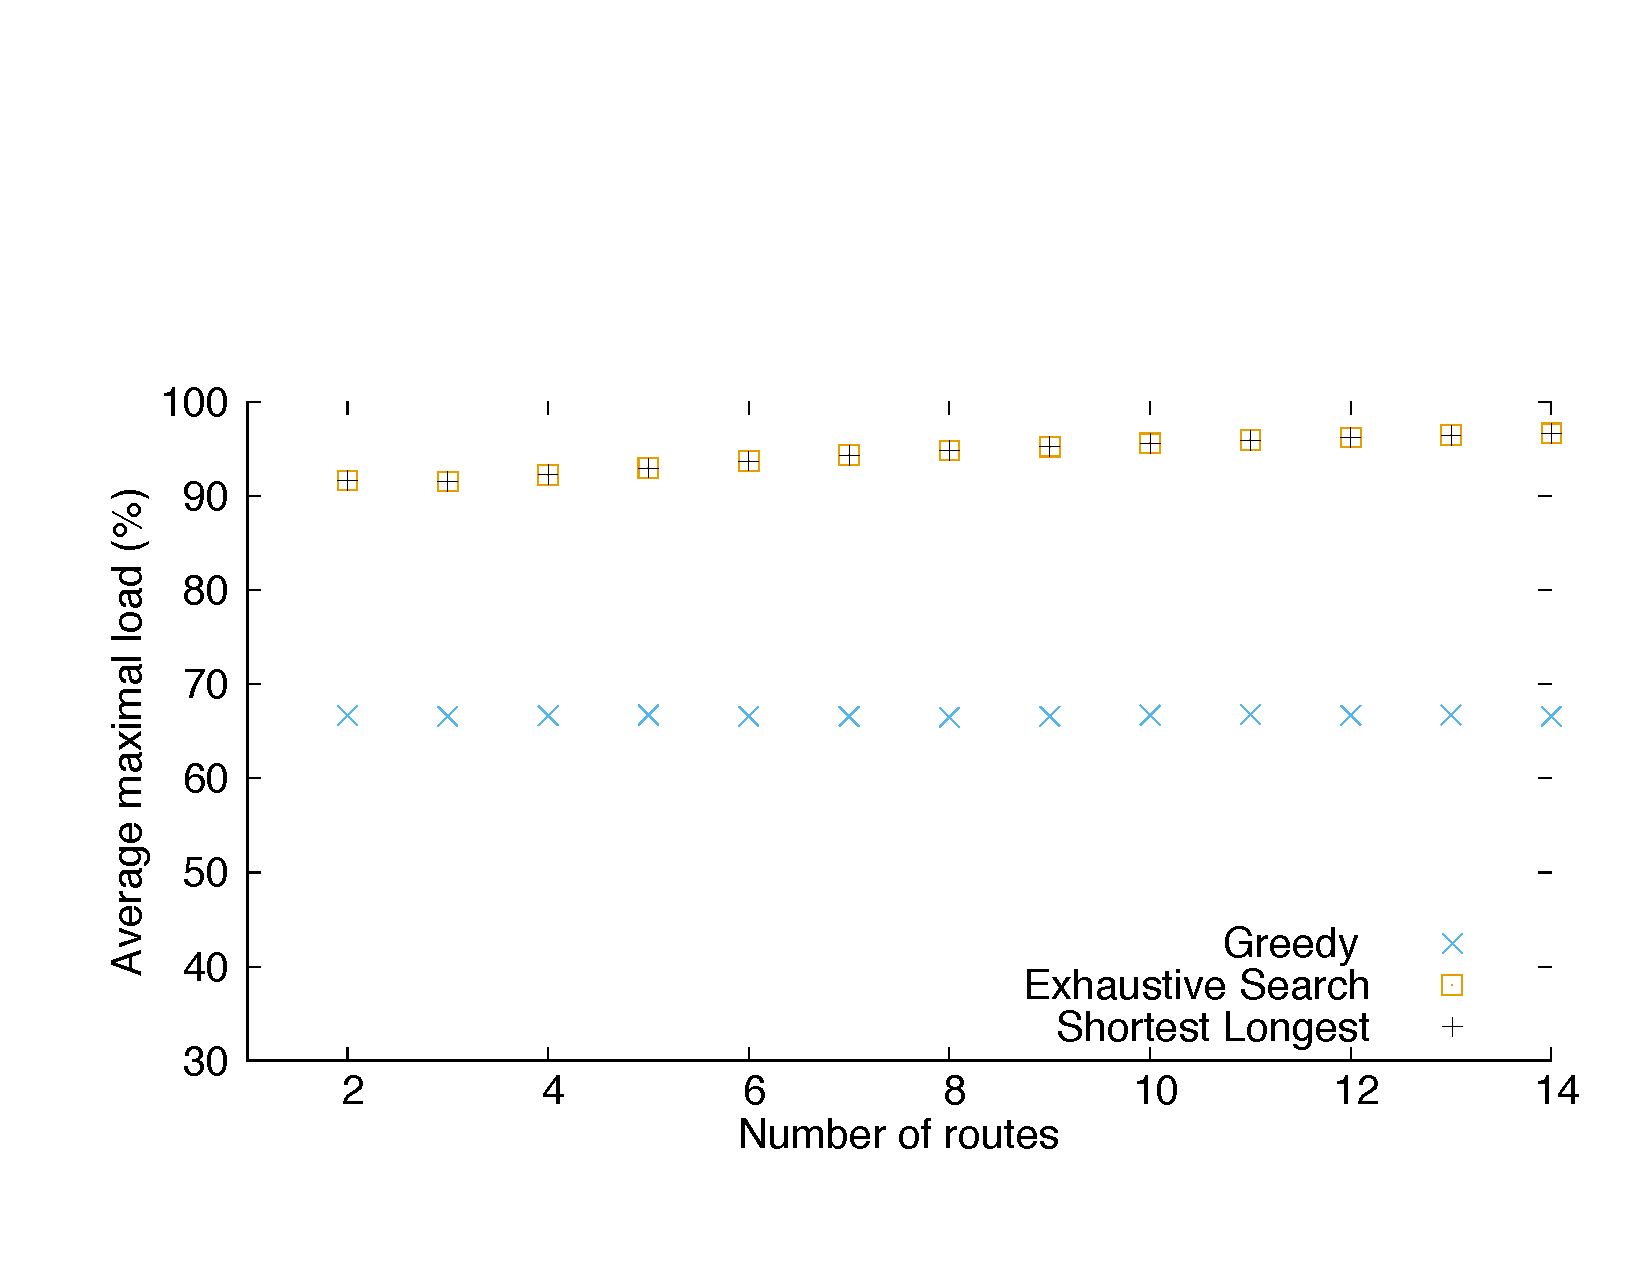
\includegraphics[width=0.47\textwidth]{periode_petite.pdf}
      \end{center}
      \caption{Maximal load averaged over $1,000$ random instances}\label{fig:short}
      \end{figure}
      First, we remark that the exhaustive search finds a solution even when the load is high, especially when there are more routes.
      It justifies the idea to look for an assignment without waiting time, in this short routes regime.
      Second, remark that the Shortest-Longest algorithm is as good as the exhaustive search. While it was expected to be good with short routes, it turns out to be optimal for all the the random star routed networks we have tried. Therefore, we should use it in practical applications with short routes, instead of the exhaustive search which is much more computationally expensive. 
      Finally, note that, on average, the greedy algorithm works when the load is less than $2/3$ which is twice better than the theoretical lower bound. This algorithm seems to depends on the load only and not on the number of routes.
      
        \paragraph{Long routes}
      
      We now want to understand the performance of these algorithms when the size of the routes is unbounded. In this experiment we fix the number of routes to $8$ and the weights of the arcs $(c_t,t_i)$ are drawn following a uniform distribution in $[P]$. We represent in Figure~\ref{fig:long} the percentage of success of each algorithm, for load from $100\%$ down to $40\%$.
      
\begin{figure}[h]

       \begin{center}
      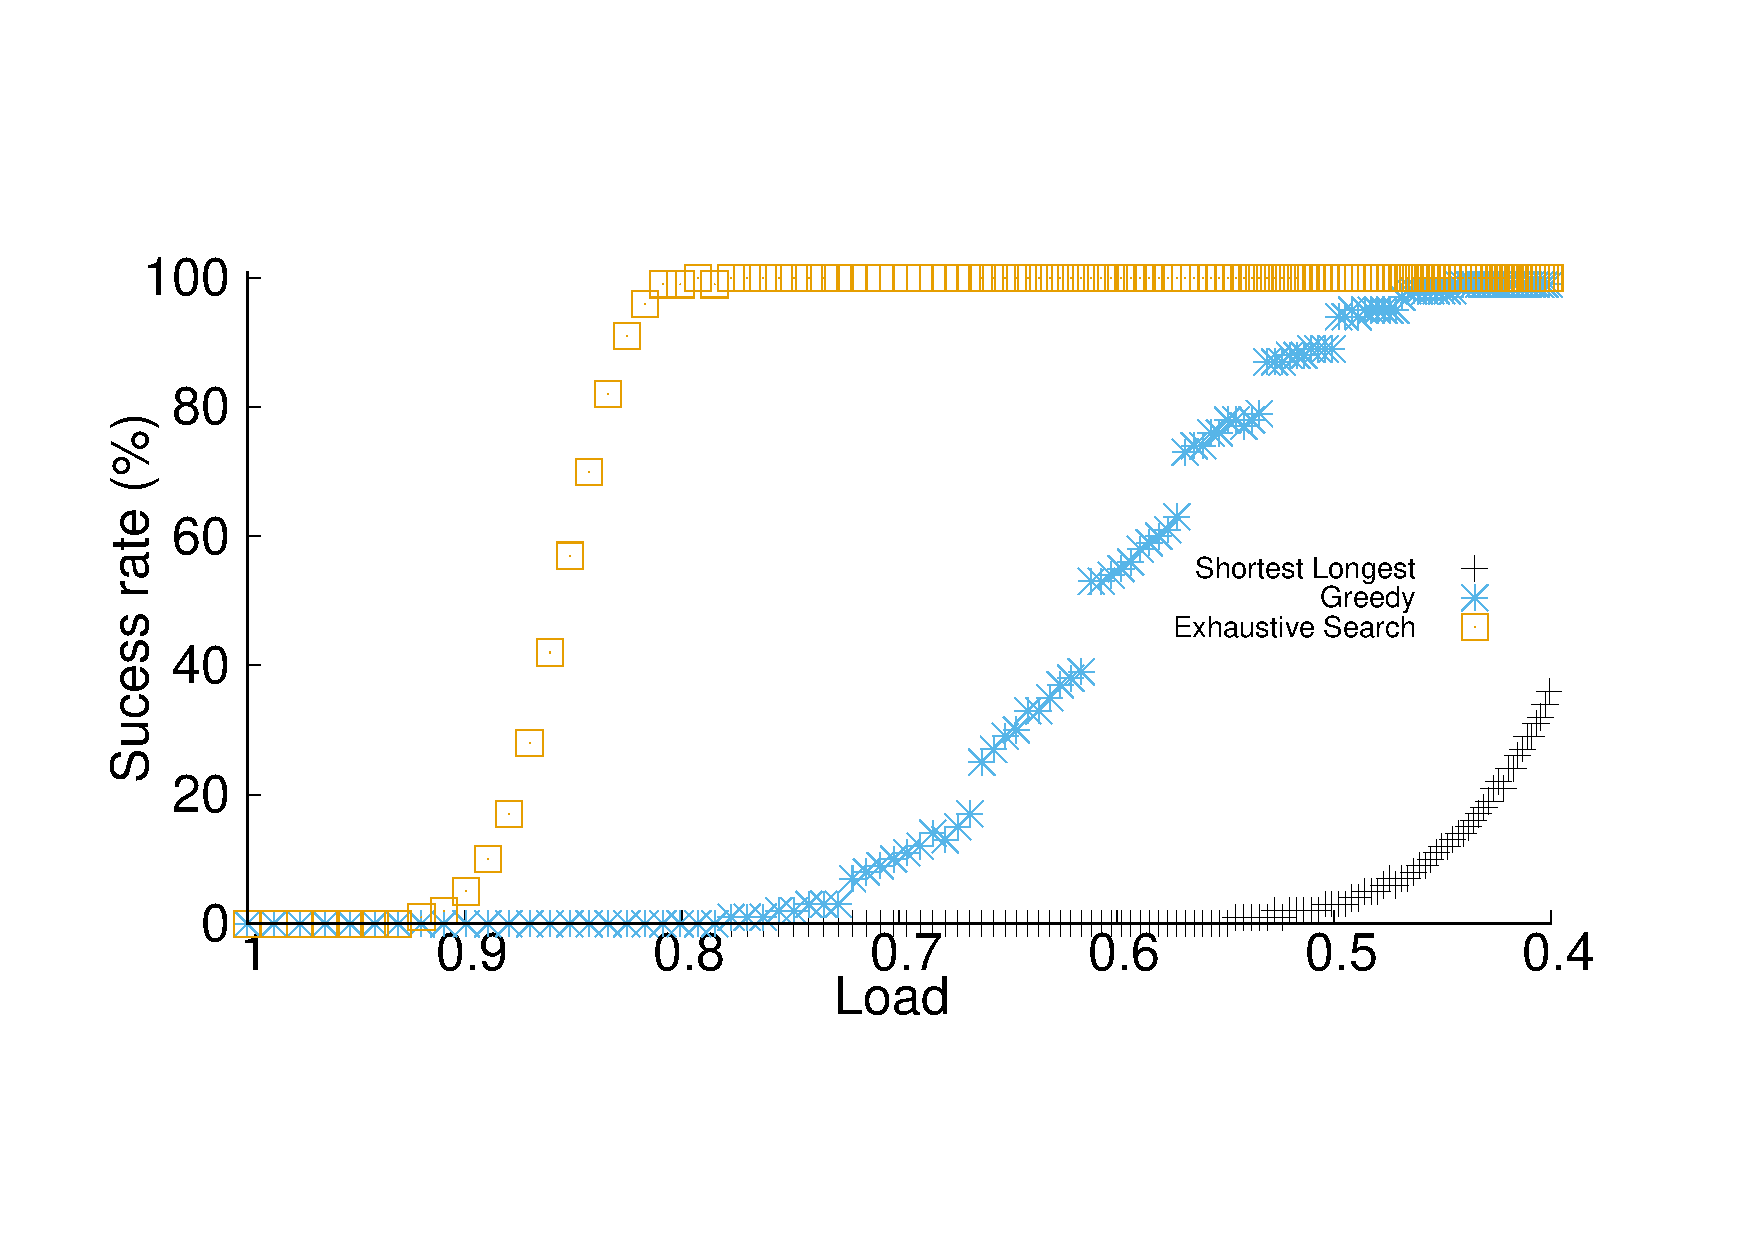
\includegraphics[width=0.47\textwidth]{echec_longues.pdf}
      \end{center}
       
      \caption{Success rate for $8$ routes over $1,000$ random instances}\label{fig:long}
     \end{figure}
      
      In this regime, the performances of Shortest-Longest are abysmal since it depends on the difference between the longest and the smallest route which is large here. On the other hand, the greedy algorithm has a performance not so far from the case of short routes, which is expected since it does not directly depend on the size of the route. In fact, if we do the previous experiment  (for short routes) but with long routes, we find that, on average, the greedy algorithm finds a solution when the load is less than $59\%$.
      
      When the load is larger than $50\%$, the exhaustive search finds more solutions than the greedy algorithms which justifies its use. However, for load larger than $80\%$ there are many instances for which there are no solutions to \pazl.
      It means that with long routes and high load, looking for an assignment without waiting time is far too restrictive. That is why we present algorithms for the general \pall problem in our next section. We will test them on $8$ long routes and a load between $100\%$ and $80\%$, parameters for which, as shown here, there are often no assignment without waiting times.
      
      The computation time of the exhaustive search is bounded by $O(n!)$ as shown in Theorem~\ref{th:FPT}, 
      but it can be much better in practice, either because it finds a solutions quickly or because a large part of the tree of 
      compact assignments is pruned during the algorithm. We study the evolution of the running time  of the algorithm when $n$ grows in the following experiment. The weights of the arcs $(c_t,t_i)$ are drawn following a uniform distribution between $0$ and $20,000$ slots. We chose  $95\%$ of load.  The table of Figure~\ref{fig:table} shows the time before the exhaustive search ends, for $8$ to $16$ routes, averaged on $100$ random star routed networks. This shows that for less than $16$ routes, which corresponds to all current topologies, the algorithm is efficient enough, but we should improve it further to work on more routes.
      
      \begin{figure}[h]
         \begin{center}
         \begin{tabularx}{0.5\textwidth}{|l|X|X|X|X|X|}
    \hline
   $n$ & $8$ & $10$& $12$&$14$& $16$\\
    \hline
   Time (s) & $6.10^{-5}$&$8.10^{-4}$&$2.10^{-2}$& $0.4$& $11$\\
    \hline
      \end{tabularx}
      \end{center}
      \caption{Running time of the exhaustive search.}
      \label{fig:table}
      \end{figure}
      
         \section{Solving \pall on Star Routed Networks}\label{sec:PALL}
    
    In this section, we consider the more general \pall problem on star routed networks. The messages are allowed to wait in the target vertices (BBUs) to yield more possible assignments. Hence, we allow the process time of a route to be greater than twice the weights of the route, but it is bounded by its deadline.

	\subsection{Simpler networks}
		
		
	Often in real networks, the length of the routes are not arbitrary and we may exploit that to solve \pall easily. For instance if all the weights on the arcs $(c_t,t_i)$ are the same, we can replace them all by $0$ and subtract this weight to the deadlines. It corresponds to a situation where all the BBUs are in the same data-center and have the same processing power. The assignment in that case is trivial, just send all messages so that they follow each other without gaps in the central arc. Since the arcs $(c_t,t_i)$ are of weight $0$, all messages will go through $(c_t,c_s)$ on their way back in the same order and thus do not collide. 
	
	Another possible assumption would be that all deadlines are sufficiently large, larger than the longest route.
	It happens when all the arcs $(s_i,c_s)$ of the original star routed network are the same or almost the same.
		
	 \begin{theorem}\label{th:asym}
	 Let $(G,{\cal R})$ be a star routed network with $n$ routes and let $P \geq n\tau$. Assume that the deadline function 
	 satisfies for all $r\in {\cal R}$, $d(r) \geq \displaystyle{\max_{r' \in  {\cal R}} 2\lambda(r')}$. Then, there is a $(P,\tau)$-periodic assignment and it can be built in time $O(n)$.
% 	 $d = \max_{i,j} |\Omega(s_i,c_s) - \Omega(s_j,c_s)$. There is a $(P,\tau)$-periodic assignment with process time $2\, \displaystyle{\max_{r\in {\cal R}} \lambda(r) + d}$ and it can be built in time $O(n)$.
	 \end{theorem}
      \begin{proof}
      W.l.o.g. say that $r_0$ is the longest route. The idea is to set the waiting times of all routes so their messages behave exactly as the message of $r_0$.        
        The offset of the forward route $r_i$ is set to $i\tau$, which ensures that there are no collisions on the arc $(c_s,c_t)$ as soon as $P \geq n\tau$ which is the minimal possible period. The waiting time of the route $r_i$ is $w_i = 2(\lambda(r_{0}) - \lambda(r_{i}))$.
        
        The time at which the message of the route $r_i$ arrives at the vertex $c_t$ on its way back is $t(c_t,\rho(r_i)) = w_i + i\tau + 2\lambda(r_{i})$. By replacing $w_i$ by its value we obtain $t(c_t,\rho(r_i)) =  i\tau + 2\lambda(r_{0})$
        As a conclusion there are no collisions on the arc $(c_t,c_s)$ as soon as the period is larger than $n\tau$ (there are no gaps between the messages). The process time of the route $r_i$ is $PT(r_i) = w_i + 2\lambda(r_{i}) $. We obtain $PT(r_i) = 2\lambda(r_{0})$ which is by hypothesis less than $d(r_i)$.
	Finally the complexity is $O(n)$ since we have to find the maximum of the length of the $n$ routes and the computation of each $w_i$ is done by a constant number of arithmetic operations.
     \end{proof}
     
    
     \subsection{A two stage approach}
     
     We can decompose any algorithm solving \pall in two parts: first set the offsets of the forward routes and then knowing this information set the offset of the backward routes or equivalently the waiting times.   
     
     First, in order to minimize the period needed to send the messages of the forward route, we set the offsets of the forward routes so that all messages have no collisions on the central arc and such that there are no free slots between the end of a message on the central arc and the beginning of the next one.
    % In the following policies, the offsets of the forward routes will be chosen so that all messages have no collisions on the central arc and such that there are no free slots between the end of a message on the central arc and the beginning of the next one. It is done to minimize the period needed to send the messages of the forward route.
     The offsets of the forward routes are then defined by the order of the messages through the central arc. We propose to study the following orders. 
	\begin{itemize}
	 
	 \item Longest-Shortest on Routes (LSR): Decreasing order on the length of the routes.
	 \item Shortest-Longest on Routes (SLR): Increasing order on the length of the routes. 
	 \item Longest-Shortest on last Arc (LSA): Decreasing order on the length of the arcs $(c_t,t_i)$.
	 \item Shortest-Longest on last Arc (SLA): Increasing order on the length of the arcs $(c_t,t_i)$. This sending order yields a $(P,\tau)$ periodic assignment in which all the $w_i = 0$, if the period is large enough (see proposition \ref{prop:SL}).
	 \item Random: A random order of the routes (RO).
	\end{itemize}

%    \todo{On peut commenter la partie suivante si on a pas fini}
    We also study another way to fix the offsets of the forward routes. Instead of packing all messages so that they follow each other
    in the central arc, we allow time between them. The order of the message is random and we consider two variations. 
    Either the time between two messages on the central arc is random and we call this policy Random Order and Random Spacing (RORS) or the space between two consecutive messages is always the same and we call this policy Random Order and Balanced Spacing (ROBS).
 	
    We denote by \bra (backward routes assignment) the problem \pall where the offsets of the forward routes are also given as input.
    In the rest of the section we will study different methods to solve \bra either by polynomial time heuristics or by an FPT algorithm. The methods to solve \bra are then combined with the proposed policies for fixing the offsets of the forward routes
    to solve \pall.  
   
   \subsection{Greedy scheduling of backward routes}
    
    Consider a forward route $r_i$, whose offset is $m_{r_i}$ and its backward route is $\rho(r_i)$.
%     We define the {\bf deadline} of $\rho(r_i)$ as $m_{r_i} + T_{max} - \Omega(s_i,c_s)$, that is the latest time at which the message can go out of $c_t$ such that $PT(r_i) \leq T_{max}$.
    We say that a backward route $\rho(r_i)$ is {\bf eligible} at time $t$ if $m_{i} +  \lambda(r_i) + \Omega(c_t,t_i) \leq t$, that is the message of the route $\rho(r_i)$ arrives at $c_t$ before time $t$ when $w_i = 0$.
    
    The first algorithm we propose to solve \bra is a greedy algorithm which sets the offset $m_{\rho(r_i)}$ of the 
    backward routes. It prioritizes the routes with the earliest deadline to best satisfy the
    constraint on the process time. Set $t=0$ and repeat the following: find $s \geq t$ the first time for which there is an eligible route with its offset not fixed. Then amongst all eligible routes at time $s$ choose the one with the smallest deadline, fix its offset to $s - \Omega(c_t,t_i) $ and set $t = s + \tau$.
    
    This algorithm does not take into account the periodicity. Say that $t_0 = t(c_t,r)$ such that $r$ is the first backward route selected by the algorithm. Then if all backward routes $r$ are such that $t(c_t,r)$ is smaller than $t_0 + P - \tau$,
    by construction, there are no collisions on the central arc.
    However, if a route $r$ has a larger $t(c_t,r)$, since we should consider everything modulo $P$, 
    it may collide with another backward route. Therefore we must adapt the greedy algorithm of the previous paragraph by finding $s \geq t$ the first time for which there is an eligible route with its offset not fixed and \emph{such that there are no collisions if a message go through the central arc at time $s$}. 
    
    Algorithm~\ref{alg:GD} is the formal description of the previous algorithm. 
     The function  min\_non\_assigned(eligible\_time) returns the non assigned route with the smallest time eligible time. The function update(t,free\_intervals) removes an interval of size $\tau$ beginning at t, which correspond to the message,  from free\_intervals.
     
      \begin{algorithm}\label{alg:GD}
     \caption{ Greedy deadline ({\bf GD}) }
     \begin{algorithmic}
     \REQUIRE A routed network $(G,{\cal R})$, a period $P$, packet size $\tau$, the deadlines $d_i$, the offsets $m_i$
     \ENSURE $(P,\tau)$-periodic assignment of $(G,{\cal R})$, or failure
    \STATE  ${\cal H} \leftarrow$ empty set //{\em set of eligible routes with their deadline}
        \STATE  free\_ intervals $\leftarrow$ [0,$P$] //{\em list of intervals of free slots}
   
     \FORALL{route $r_{i}$}
%      \STATE  deadline[$r_i$]  $\leftarrow$  $m_{i} + T_{max} - \Omega(s_i,c_s)$
     \STATE  eligible\_time[$r_i$] $\leftarrow$ $m_{i} +  \lambda(r_i) + \Omega(c_t,t_i)$
       \ENDFOR
       
       \WHILE{There is some non-assigned routes}
       \IF{${\cal H}$ is empty}
       \STATE $r_i$ $\leftarrow $ min\_non\_assigned(eligible\_time)
       \STATE insert(${\cal H}$,$r_i$,$d_i$).
       \ENDIF
      
       \STATE $r \leftarrow $ extract\_min(${\cal H}$)
       \STATE t $\leftarrow$ next\_free\_interval(free\_intervals, t) //{\em if there is no more free interval of size $\tau$, the algorithm fails}
       \STATE $w_i \leftarrow$ t - eligible\_time[$r_i$]
       \STATE update(t,free\_ intervals)
       \STATE t $\leftarrow$ t + $\tau$
       \FORALL{routes $r_i$ with  eligible\_time[$r_i$] $\leq$ t}
 \STATE insert(${\cal H}$,$r_i$).
       \ENDFOR
       \ENDWHILE
     \end{algorithmic}
     \end{algorithm}


    The complexity of Algorithm~\ref{alg:GD} is in $O(n\log(n))$, using the proper data structures.
    The set of eligible routes must be maintained in a binary heap
    to be able to find the one with smallest deadline in time $O(\log(n))$. 
    To deal with the possible collisions, one maintains a list of the intervals
    of time during which a message can be sent on the arc $(c_t,c_s)$. Each time the offset of a 
    route is fixed an interval is split into at most two intervals in constant time. 
    Since the algorithm goes over the elements of this list at most twice when doing an insertion
    or looking for the next free interval, the time needed to maintain it is $O(n)$. 
  
     \subsection{Earliest deadline scheduling}\label{sec:braheuristic}
     
     
     The problem \bra is the same as the following scheduling problem if we forget the periodicity. Given a set of jobs with \emph{release times} and  \emph{deadlines}, schedule all jobs on a single processor, that is choose the time at which they are computed, so that no two jobs are scheduled at the same time. A job is always scheduled after its release time and it must be finished before its deadline. Let us call $n$ the number of jobs, the problem can be solved in time $O(n^2\log(n))$~\cite{simons1978fast} when all jobs have the same running time and it gives a solution which minimizes the time at which the last job is scheduled. On the other hand if the running times are different the problem is $\NP$-complete~\cite{lenstra1977complexity}. 
     The  polynomial time algorithm  which solves this scheduling problem is similar to the greedy algorithm presented in the previous section. However, when it fails because a job finishes after its deadline, it changes the schedule of the last messages to find a possible schedule for the problematic job. The change in the scheduling is so that the algorithm cannot fail on the same job a second time except if there are no solutions, which proves that the algorithm is in polynomial time.
     
     The problem \bra is reduced to this scheduling problem. The backward routes are the jobs, the size of a message is the running time of a job, the deadline of a route is the deadline of the corresponding job and the smallest time at which it is eligible is the release time. Let us call {\bf Minimal Latency Scheduling (MLS)} the algorithm which transforms \bra into the described scheduling problem to solve it in polynomial time.
     
     Let us denote by $y_i$ the time at which the message of the route $r_{\rho(i)}$ cross the node $c_t$,
     that is $y_i = m_{\rho(i)} + \lambda(i)$. Let us denote by $y_{min}$ and $y_{max}$ the smallest and largest value of the $y_i$'s. When MLS finds an assignment $m$, it always satisfies $PT(r) < d(r)$ for all $r$. If $y_{max}- y_{min} \leq P -\tau $, then all messages cross $c_t$ in the same period and 
     the scheduling algorithm guarantes that there are no collision. However, if $y_{max}- y_{min} > P -\tau $, then we must take into account the periodicity by computing the $y_i$ modulo $P$ and the solution we obtain by MLS may have a collision. Since the scheduling algorithm minimizes $y_{max}$, it may work sometimes (as shown in Section~\ref{sec:resultsPALL}), but not for all instances. 
     
     
     We now present a variant of the previous algorithm that we call {\bf Periodic Minimal Latency Scheduling (PMLS)}. The aim is to deal with the periodicity, by modifiying the instance (without changing the assignments) so that the chance of finding a solution with $y_{max}- y_{min} \leq P -\tau $ are larger.  Remark that if an instance has a satisfying assignment, we can always guarantee that one route has a waiting time zero in a satisfying assignment. Hence, there is a route, which can be considered as the first one (release time $0$) and we may assume it has zero waiting time.
     
     Algorithm PMLS runs, for each route $r$, the algorithm MLS on an instance defined as follows. 
     Let $RT(r)$ be the release time of $r$, we subtract it to all release times and deadlines.
     Therefore $RT(r)$ is zero in this instance and the time at which the message of $r$ crosses $c_t$ is also set to zero, hence its waiting time is zero.  We then modify the instance so that all release times are in $[P-\tau]$: Each release time $RT(r_i)$ is replaced by $RT(r_i) \mod P$ and $RT(r_i) - (RT(r_i) \mod P)$ is subtracted to the deadline $d(r_i)$. Furthermore, if a release time of a route $r_i$ is between $ P-\tau$ and $P$, we set it to $0$ and $d(i) = d(i) - P$. 
     
     The deadline of each backward route is set to the minimum of their deadline and $P - \tau$. Because of this modification of deadlines, if MLS finds a solution for an instance, we have $y_{max}- y_{min} \leq P -\tau $, hence it is a $(P,\tau)$ periodic assignment.  The algorithm PMLS finds periodic assignments more often than MLS, because if MLS finds a solution with $r_i$ the route such that $y_i = y_{min}$, then this solution is found by PMLS when it selects $r_i$ as the first route. Since MLS is used at most $n$ times, the complexity of PMLS is in $O(n^3\log(n))$. Note that PMLS is a heuristic and may fail if all assignments have some $y_i$ larger than $P - \tau$.
     
%     \begin{algorithm}[H]
%     \caption{ Minimized Scheduling Periodic (MSP)}
%     \begin{algorithmic}
%     \REQUIRE A routed network $(G,{\cal R})$,a period $P$, packet size $\tau$, $ T_{max}$, the offsets $m_i$
%     \ENSURE $(P-\tau)-$periodic assignment of $(G,{\cal R})$, if it exists
%   
%     \FORALL{route $r_{t_i}$}
%     \STATE  $w_i \leftarrow 0$
%     \STATE period-end $\leftarrow m_{s_i} + \lambda(r_{s_i}) + t(c_t,r_{t_i}) + P$
%     \FORALL{route $r_{t_j}$}
%     \STATE deadline-route$ \leftarrow m_{s_j} + T_{max}-t(c_s,r_{s_j})$
%     \STATE $deadline \leftarrow$ min(deadline-route,period-end)
%     \ENDFOR
%     
%     \STATE Call (MS)
% 
%     
%     \ENDFOR
% 
%     \STATE return the best $(P,\tau)$-periodic assignment, or FAILURE
% 
%     \end{algorithmic}
%     \end{algorithm}

\subsection{FPT algorithms for \bra and \pall}

As a warm-up, we give a simple FPT algorithm for \bra which is practical,
and then we build on it to give a more complicated FPT algorithm for \pall. Unfortunately, the dependency on $n$ the number of routes in the second algorithm is yet too large to be useful in practice. 

\begin{theorem}\label{th:braFPT}
$\bra \in \FPT$ when parametrized by the number of routes.
\end{theorem}
\begin{proof}
 Consider an instance of \bra, which can be characterized by a release time and a deadline for each route.
 We will show that we can create a set of instances such that one of these instances has an assignment if and only if the original instance has an assignment. As for PMLS, for each route $r_j$, we consider the instance where $r_j$ has release time and waiting time zero ($RT(r_j) = y_j = 0$). The release times and deadlines of all routes are changed so that all release times are less than $P$ as in the transformation described for PMLS. If there is an assignment such that for all $i$, $y_i < P-\tau$, then the periodicity does not come into play for this assignment and the algorithm MLS will find it as explained in Section~\ref{sec:braheuristic}.

 Now, remark that if there is a periodic assignment for an instance, then there is a periodic assignment satisfying for all $i$, $y_i \leq 2P - \tau$.  Indeed, if there is a $i$ such that $y_i > 2P$ in
a periodic assignment, then setting $y_i = y_i - P$ cannot create a collision and improve the 
process time of $r_i$ by $P$. Since $y_i - P > P$, it is a valid assignment, that is the route $r_i$ sends its message after its release time. Moreover, for all $i \neq j$, it is not possible that $2P-\tau < y_i \leq 2P$, since by construction $y_j = 0$ and it would induce a collision.
 

From a periodic assignment satisfying that for all $i$, $y_i \leq 2P - \tau$, we define 
a new instance whose periodic assignments are a subset of the periodic assignments of the original instance. Moreover, one of the periodic assignments of the new instance satisfies for all $i$, $y_i \leq P - \tau$ and will thus be found by MLS. Let $S$ be the set of routes $r_i$ such that  $P - \tau < y_i \leq 2P - \tau$. The new instance is defined by setting the release time of the routes in $S$ to $0$ and by subtracting $P$ to their deadlines. Then the considered periodic assignment is a solution of the new instance with all $y_i \leq P -\tau$. Moreover any solution of the new instance is a solution of the original one, since we have made the constraints harder.   

The FTP algorithm is the following: for each subset $S$ of routes, remove $P$ to the release time and to the deadline of each route in $S$ and run MLS on the new instance. If there is an assignment, then we have proved that there is an $S$ such that the modified instance has a solution with all messages going through the central arc between $0$ and $P - \tau$, a solution that MLS will find.
\end{proof}

The algorithm of Theorem~\ref{th:braFPT} has a complexity of $O(2^nn^3\log(n))$. Moreover, for each backward route to be scheduled between $P$ and $2P-\tau$, it must have a deadline larger than $P + \tau$ since between $P$ and $P + \tau$ the first message goes through the central arc. Often, only a small fraction of the routes have a deadline larger than $P + \tau$, say $k$ of them and we explore only $2^k << 2^n$ cases. Let us call this algorithm {\bf FPT-PMLS} for the rest of the article.


\begin{theorem}\label{th:pallFPT}
$\pall \in \FPT$ when parameterized by the number of routes.
\end{theorem}
\begin{proof}
 Consider an instance of \pall which has a solution. We now characterize such a solution by a set of necessary and sufficient linear equations and inequations it must satisfy. 
 For simplicity, we consider $x_i$ the time at which a message goes through $c_t$ on the forward route $r_i$ and $y_i$ the time at which it goes through $c_t$ on the backward route $r_{\rho(i)}$.
 Choosing values for $x_i$ and $y_i$ is equivalent to choosing the offsets $m_i$ and $m_{\rho(i)}$.
 
 The values $x_i$ and $y_i$ satisfies the following inequation: $y_i \geq x_i + 2\lambda(r_i)$.
We may assume that the first route has release time and waiting time zero, 
that is $x_0 = y_0 = 0$. We can also guarantee that all $x_i$ are less than $P-\tau$ if we modify
the release times and deadlines without changing the possible assignments. As in Theorem~\ref{th:braFPT}, we have all $y_i < 2P - \tau$,
and  when $y_i \geq P - \tau$ we replace $y_i \geq x_i + 2\lambda(r_i) $ by $y_i \geq x_i + 2\lambda(r_i) - P$ and we replace the deadline $d(r_i)$ by $d(r_i) -P$. In that way we guarantee that all $y_i$ are less than $P-\tau$.  
 
 Since all $x_i$ and $y_i$ are in $[P-\tau]$, taking the values of $x_i$ and $y_i$ modulo $P$
 does not change anything, which makes easy to express the absence of collisions between routes.
 To express that there are no collision between forward routes, the following equations must be  satisfied: for all $i$, $x_i + \tau \leq x_{i+1}$. We assume that the routes are here indexed such that the $x_i$ are in ascending order.
 Let $\sigma : [n] \rightarrow [n]$ be the permutation such that the $y_{\sigma(i)}$ are in ascending order.
 To express that there are no collision between backward routes, the following equations must be  satisfied: for all $i$, $y_{\sigma(i)} + \tau \leq y_{\sigma(i+1)}$. Finally, the deadline of each route must be respected, that is for each $i$, $y_i \leq d(r_i)$. 

 Let $S$ be the system of all the previous equations, by construction of $S$, any of its solutions seen as a choice of offsets is an assignment since there are no collisions in the forward and backward period between $0$ and $P$ and we have guaranteed that all routes meet their deadlines. However, the solutions of $S$ may have rational values, while offsets must be integers. 
Remark that $x +e_1 \leq y + e_2$ implies $\lceil x \rceil +e_1 < \lceil y \rceil + e_2$ when $e_1$ and $e_2$ are integers. Therefore, since all the inequations and equations of $S$ have this form, if we take the upper floor of the values of a solution of $S$, it is still a solution of $S$ with \emph{integer} values. As a consequence, any rounded solution of $S$ yields a solution of the considered instance of \pall.

Now remark that the construction of $S$ depends on the choice of the order of the forward routes, the order of the backward routes, and on the choice of the backward routes where $P$ has been subtracted from the offset. Hence to solve \pall, we must solve $2^n(n!)^2$ systems with $2n$ variables and a bitsize of the same order than the instance of \pall. Since solving each system can be done in polynomial time it proves the theorem.
\end{proof}


    \subsection{Experimental evaluation}
    \label{sec:resultsPALL}
    \subsubsection{Performances on random topologies }
    
    We set the number of routes to $8$ to make comparisons with the results of Section~\ref{sec:exp_PAZL} easier. 
    We draw uniformly the weights of the arcs between $0$ and $20,000$. To simplify the experiments, 
    we use \emph{the same deadline} for all routes. We define the {\bf margin} as the difference between the deadline and twice the longest route. The margin represents the \emph{logical latency} imposed by the communication process without taking into account the physical length of the network which cannot be changed. For a given star routed network, setting the margin or the deadline is the same, but when comparing different star routed networks with different size of routes, the margin is more relevant than the deadline.
    In our experiments the margin ranges from  $0$ to $3,000$.
   We look at two different regimes, a medium load of $80\%$ and a high load of $95\%$.
   Considering smaller load is not relevant since we can solve the problem without waiting times as shown in Section~\ref{sec:exp_PAZL}. 
   
   We first try to understand what is the best choice of order for the first stage of the algorithm which is followed by the GD algorithm in this experiment. In Figure~\ref{fig:success80} and \ref{fig:success95}, we represent the success rate of the seven kind of orders with regards to the margin. The value is an average computed over $10,000$ random star routed networks. For RO, RORS and ROBS, we draw $1000$ random orders and count it as a success as soon as there is a solution for one order. Each random order drawn is used for RO, RORS and ROBS to make the comparison fairer.
   

\begin{figure}[h] 
  \centering
          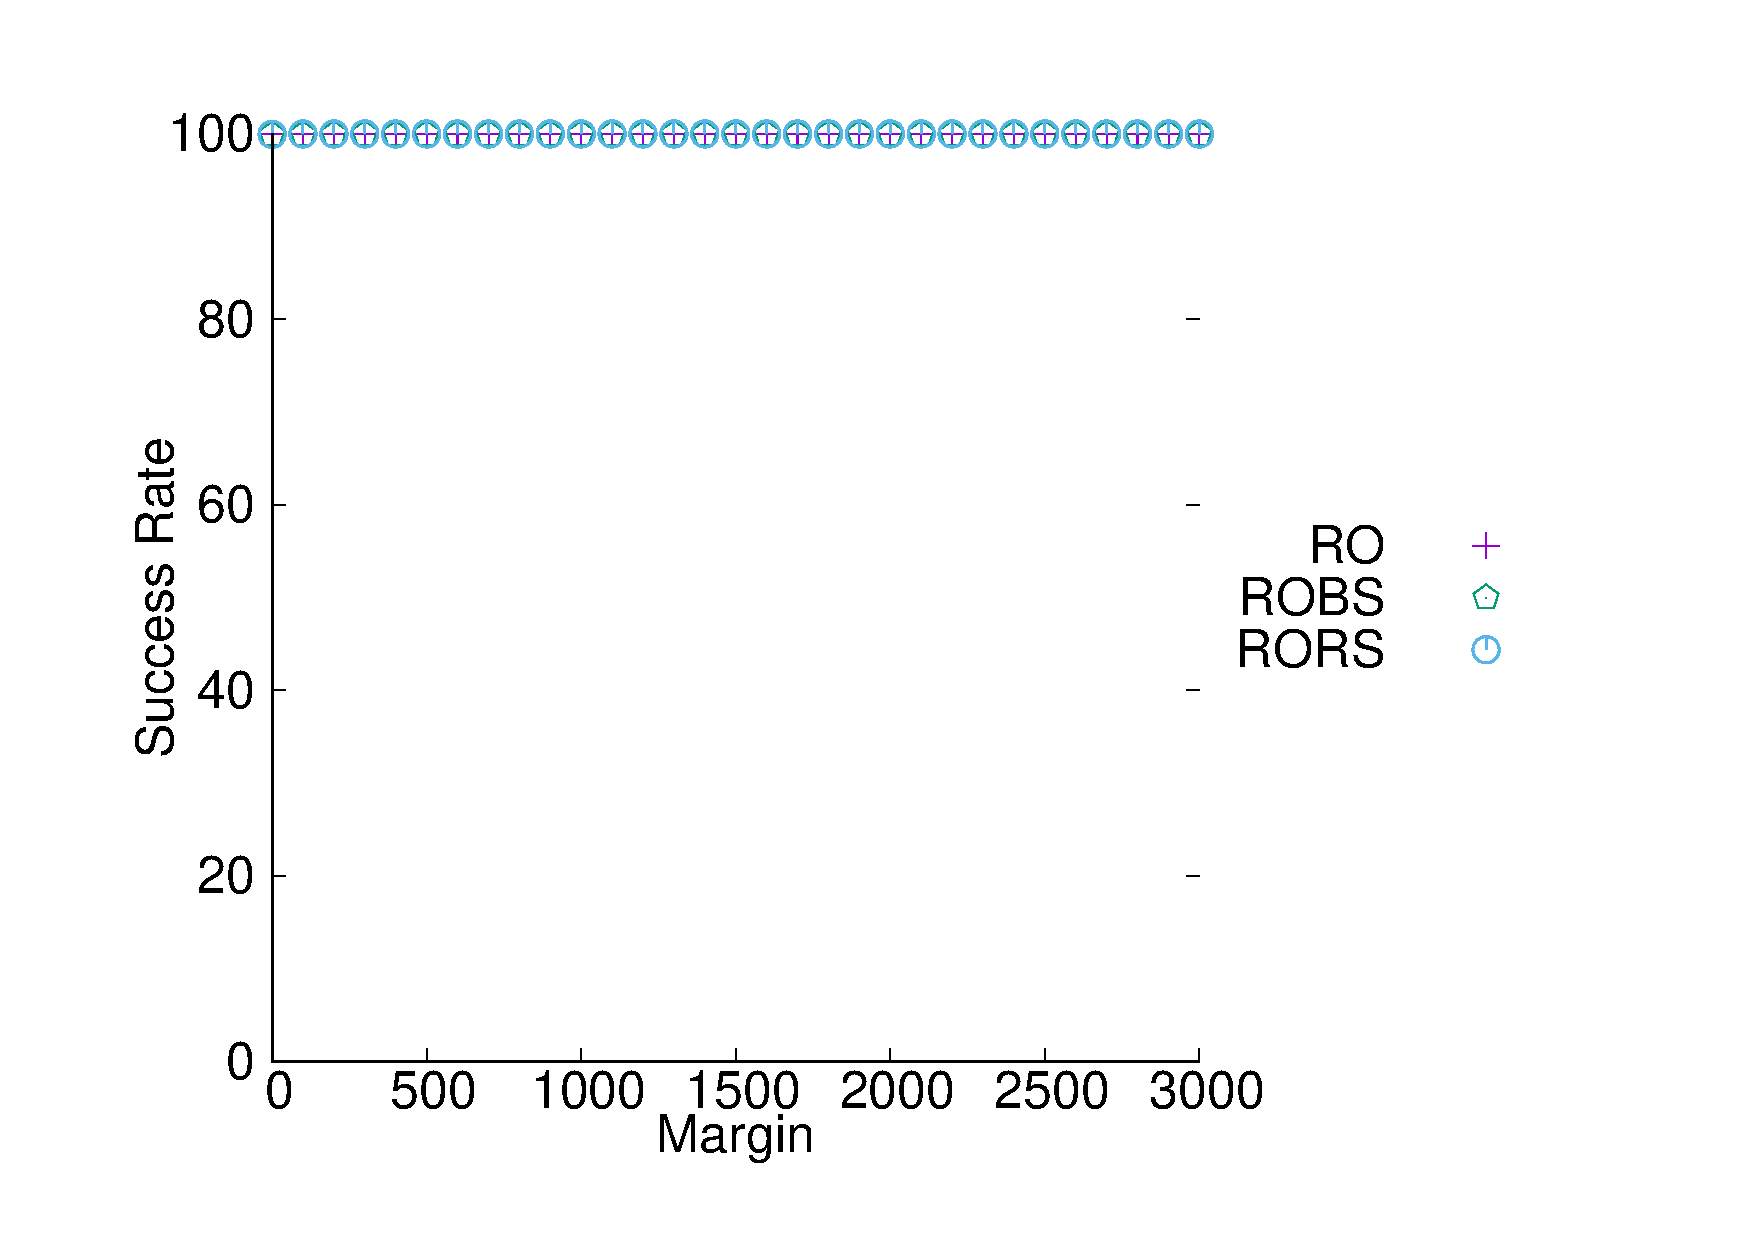
\includegraphics[width=0.5\textwidth]{departs_gp_25000.pdf}
      \caption{Success rate of different sending orders, $80\%$ load.}
           \label{fig:success80}
     \end{figure}
     
\begin{figure}[h] 
  \centering
    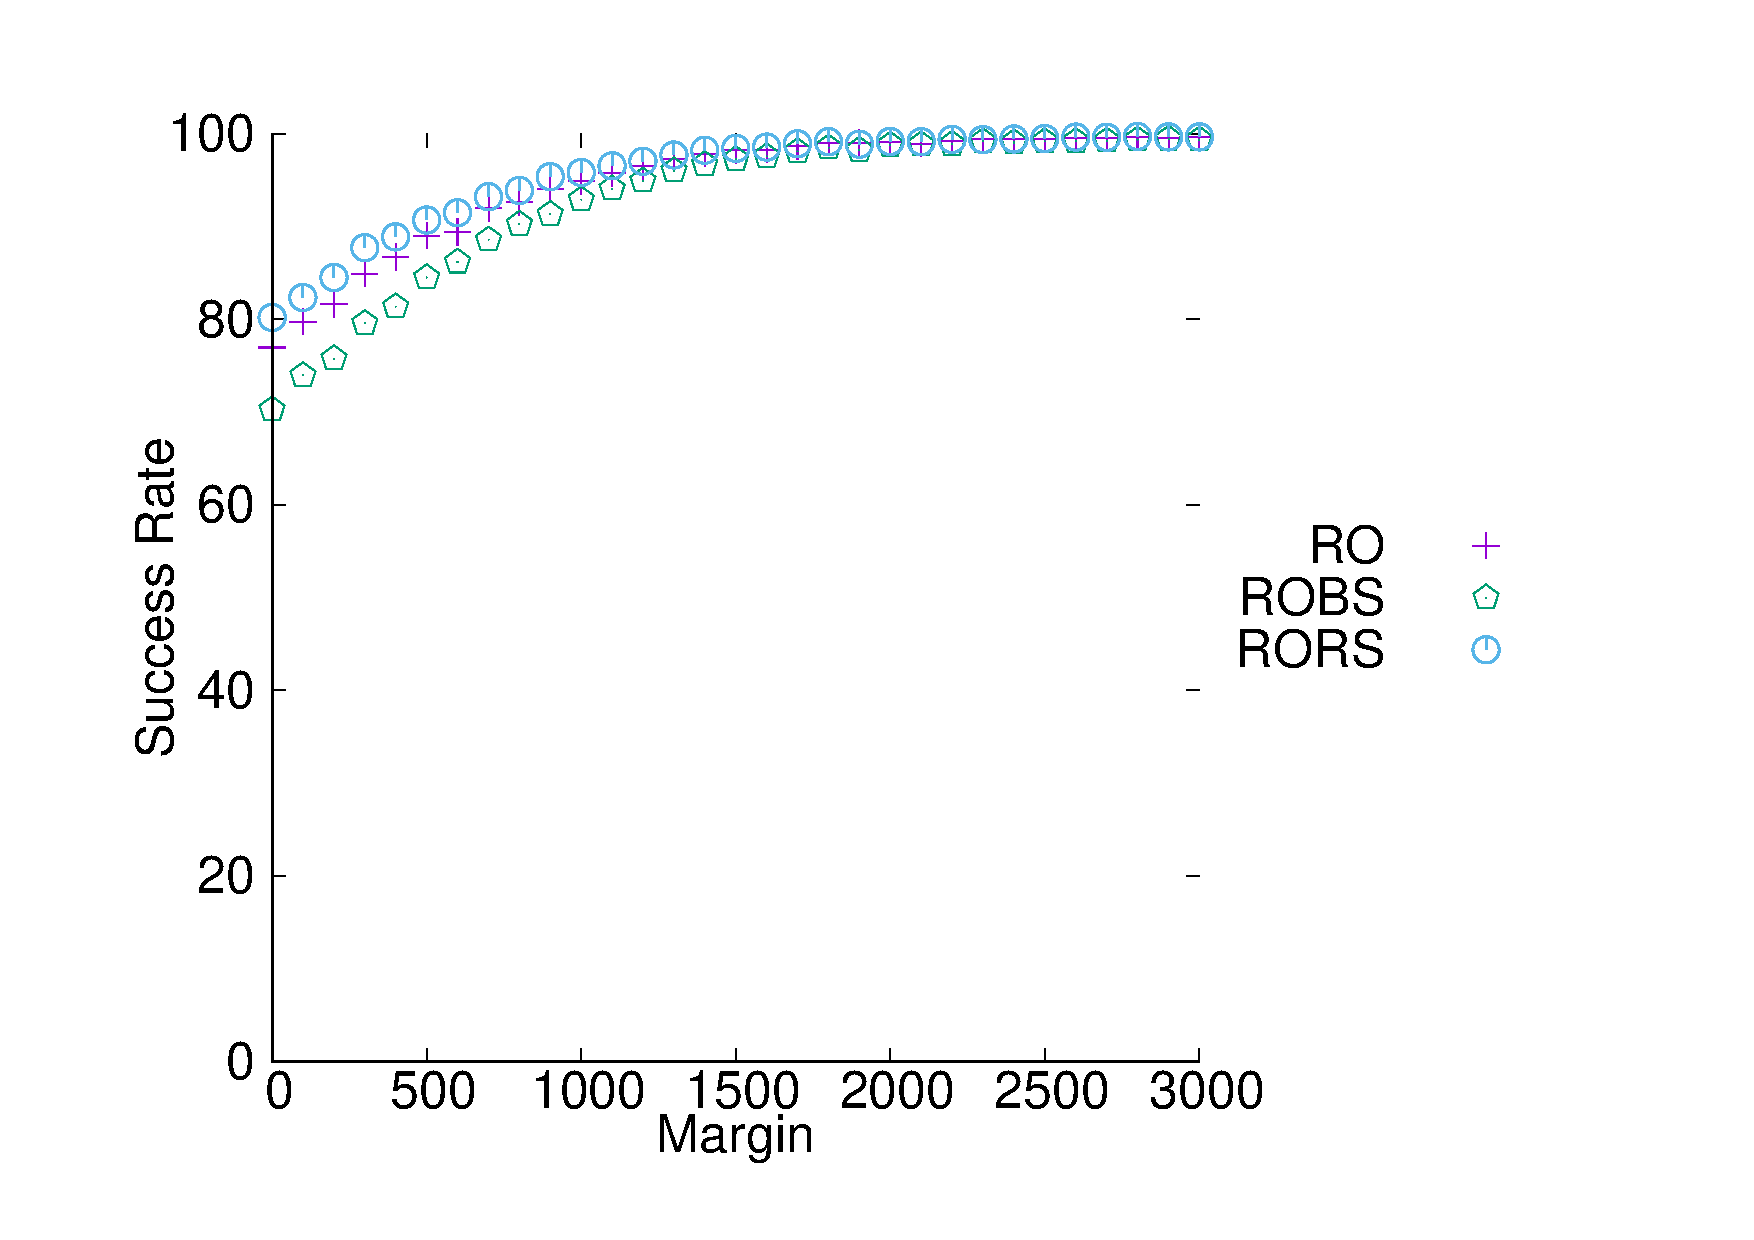
\includegraphics[width=0.5\textwidth]{departs_gp_21000.pdf}
      \caption{Success rate of different sending orders, $95\%$ load.}
      \label{fig:success95}
          \end{figure}

     First remark that our algorithms often finds assignments for $95\%$ of load and long routes which was not possible 
     when disallowing waiting times (see Section~\ref{sec:exp_PAZL}). It justifies the interest of studying \pall rather than \pazl.
          
     According to our experiments, sending the messages from the shortest to the longest route or arc does not work well. It corresponds to the policy of Proposition~\ref{prop:SL} which we already know to be bad for \pazl when the routes are long as in this experiment. Sending from the longest to the shortest route or arc works better and it seems that sorting the routes according to the length of the last arc rather than the route is better, at least in a loaded network. 
     
     Using many random orders is much better than our arbitrary choices of order. With a load of $95\%$, a solution is found with margin $0$ most of the time. The three random order policies have similar performances, but RO gives slightly more solutions than the two others ones, under high load and small margin. Hence, in the following experiments, we will always draw $1,000$ random orders using the policy RO to set the offsets of the forward routes.
     
      We now compare the performances of the four different algorithms used in the second stage. Since GD already finds assignments with margin $0$ on mild loads, it is more interesting to focus on the behavior of the algorithms with high load. In Figure~\ref{fig:success21000}, we represent the success rate of the four algorithms with regards to the margin,  computed over $10,000$ random star routed networks generated with the same parameters as previously. 
     
    \begin{figure} [h] 
       \begin{center}
      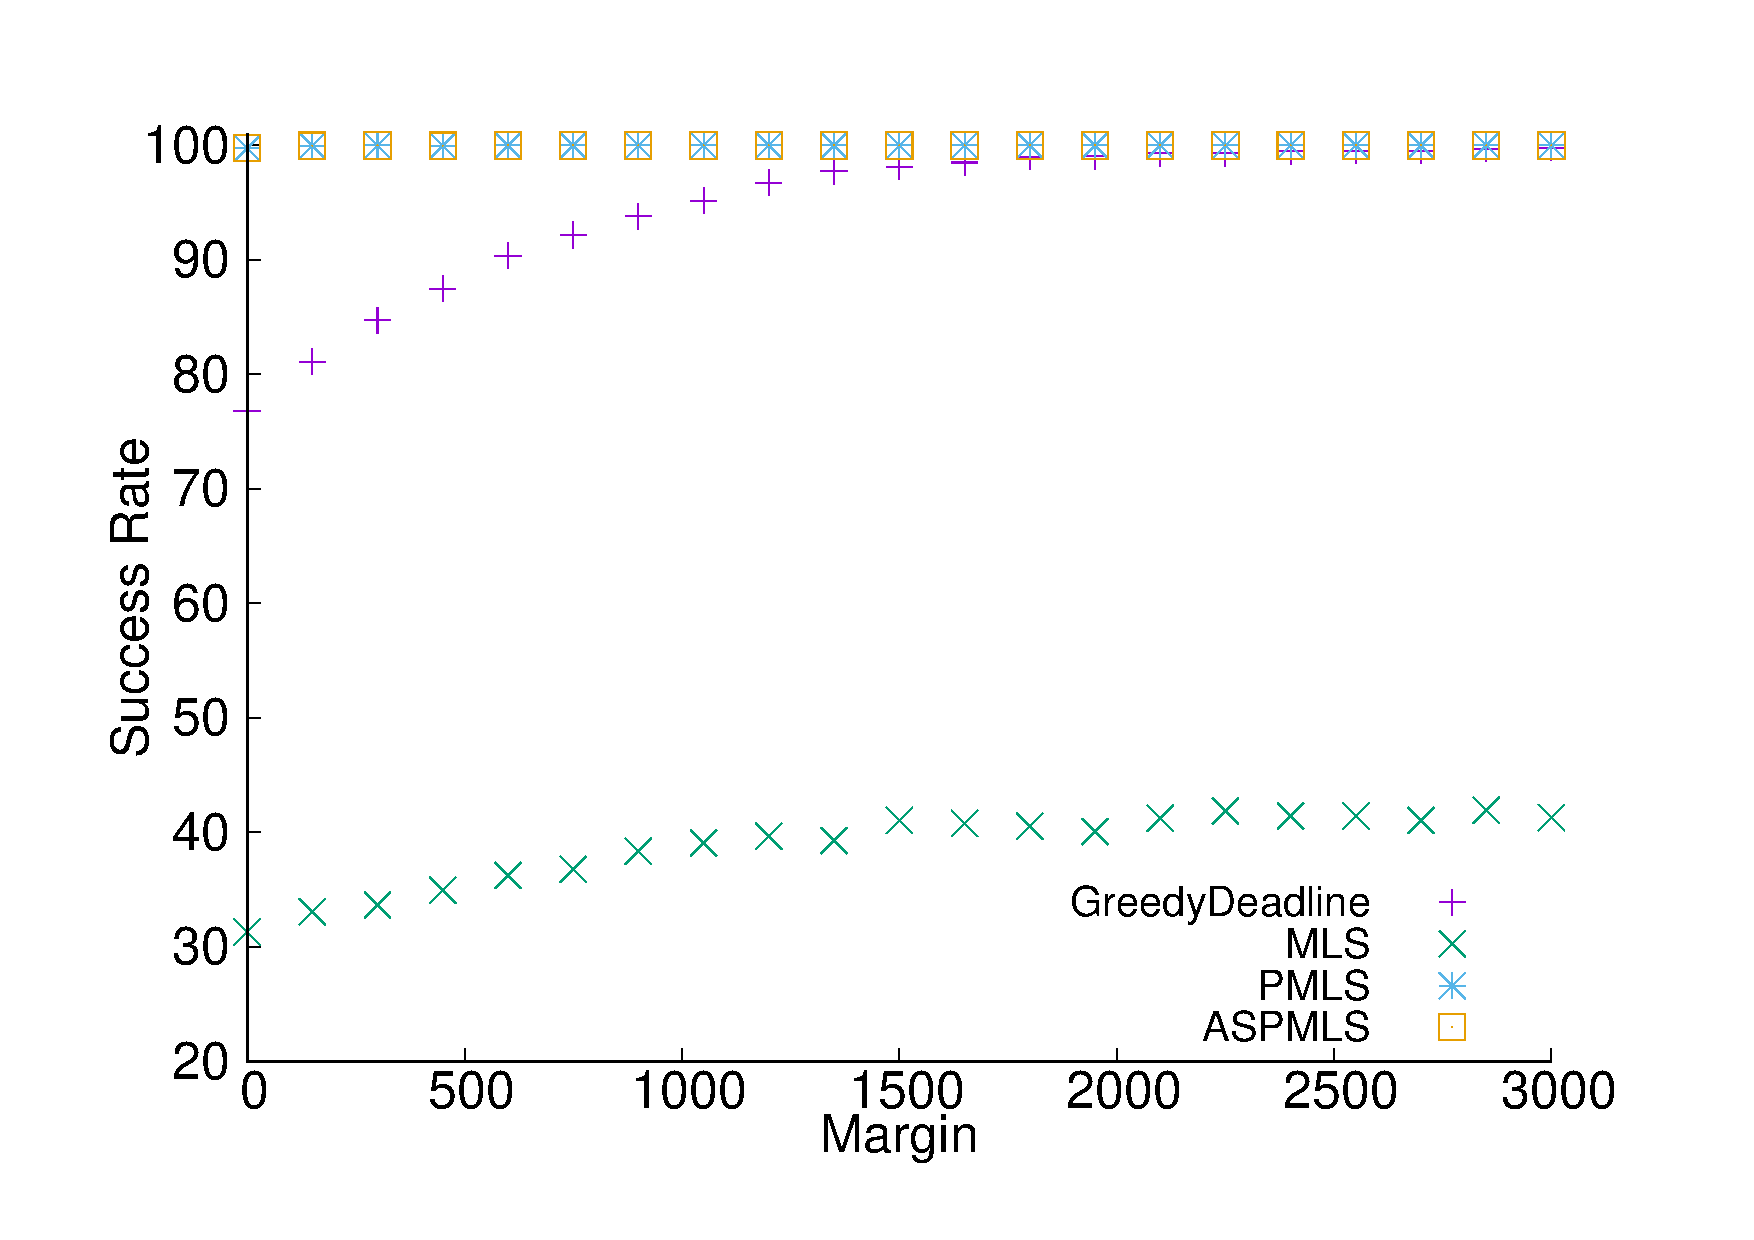
\includegraphics[width=0.5\textwidth]{retour_21000.pdf}
      \end{center}
      \caption{Success rate of GD, MLS, PMLS and FPT-PMLS, $95\%$ load}
     \label{fig:success21000}
     \end{figure}
     
      The MLS algorithm performs poorly, worst than GD, PMLS and FPT-PMLS, which shows that \emph{taking into account the periodicity} is fundamental.
     The GD algorithm is close to $100\%$ success rate for margins larger than $1,500$ while the PMLS and FPT-PMLS algorithms find a solution for more than $99\%$ of the random instances, even \emph{with a margin $0$}. In other words, for very high load and no margin, there are very few instances for which we do not find an assignment. With a margin of $300$, which corresponds to about $15\mu$s of additional delay with the chosen parameters, we always find a solution. 
     
     It turns out that the performances of PMLS and FPT-PMLS 
     are almost identical. Even with a load of $100\%$ and a margin of $0$, we have to draw $100,000$ random instances before finding one which can be solved by FPT-PMLS and not by PMLS. Since FPT-PMLS is of exponential complexity in $n$, it does not seem relevant to use it. We now present the computing time of PMLS and FPT-PMLS to understand the size of instances which can be solved. To stress the algorithms, we set the margin to $0$ and the load to $95\%$. The table on Figure~\ref{fig:tps_fpt} shows the computation times of PMLS and  FPT-PMLS, averaged on $1,000$ instances. 
     
          \begin{figure}[h] 
       \begin{center}
   \begin{tabularx}{0.5\textwidth}{|c|X|X|X|X|X|X|}
    \hline
    \# routes& $8$ & $12$ & $16$& $20$ & $24$\\
    \hline
    FPT-PMLS (ms) & $1.88$ &$5.98$&$47.75$&$209.2$&$1815$\\
    \hline
     PMLS (ms) & $0.07$ &$0.08$&$0.09$&$0.10$&$0.12$\\
    \hline
 Ratio & $27$ &$78$&$523$&$2122$&$14882$\\
    \hline
      \end{tabularx}
      \end{center}
   \caption{Computing time of PMLS and FPT-PMLS with regard to the number of routes}
        \label{fig:tps_fpt}
     \end{figure}
    
  The complexity of both these algorithm depends on the number of routes. As shown in Figure~\ref{fig:tps_fpt}, the time complexity of PMLS seems linear on \emph{average}, while its theoritical worst case complexity is cubic. FPT-PMLS scales exponentially with the number fo routes as expected. Both algorithms are usable for instances of $20$ routes, but for $40$ routes or more,  FPT-PMLS becomes too slow. Since FPT-PMLS almost never finds a solution when PMLS does not and is much slower, one should always prefer to use PMLS. 
  
%     Figure~\ref{fig:exec_time} shows the average computation time of the two algorithms during the previous experiment.
%     
%        \begin{figure} [h] 
%       \begin{center}
%      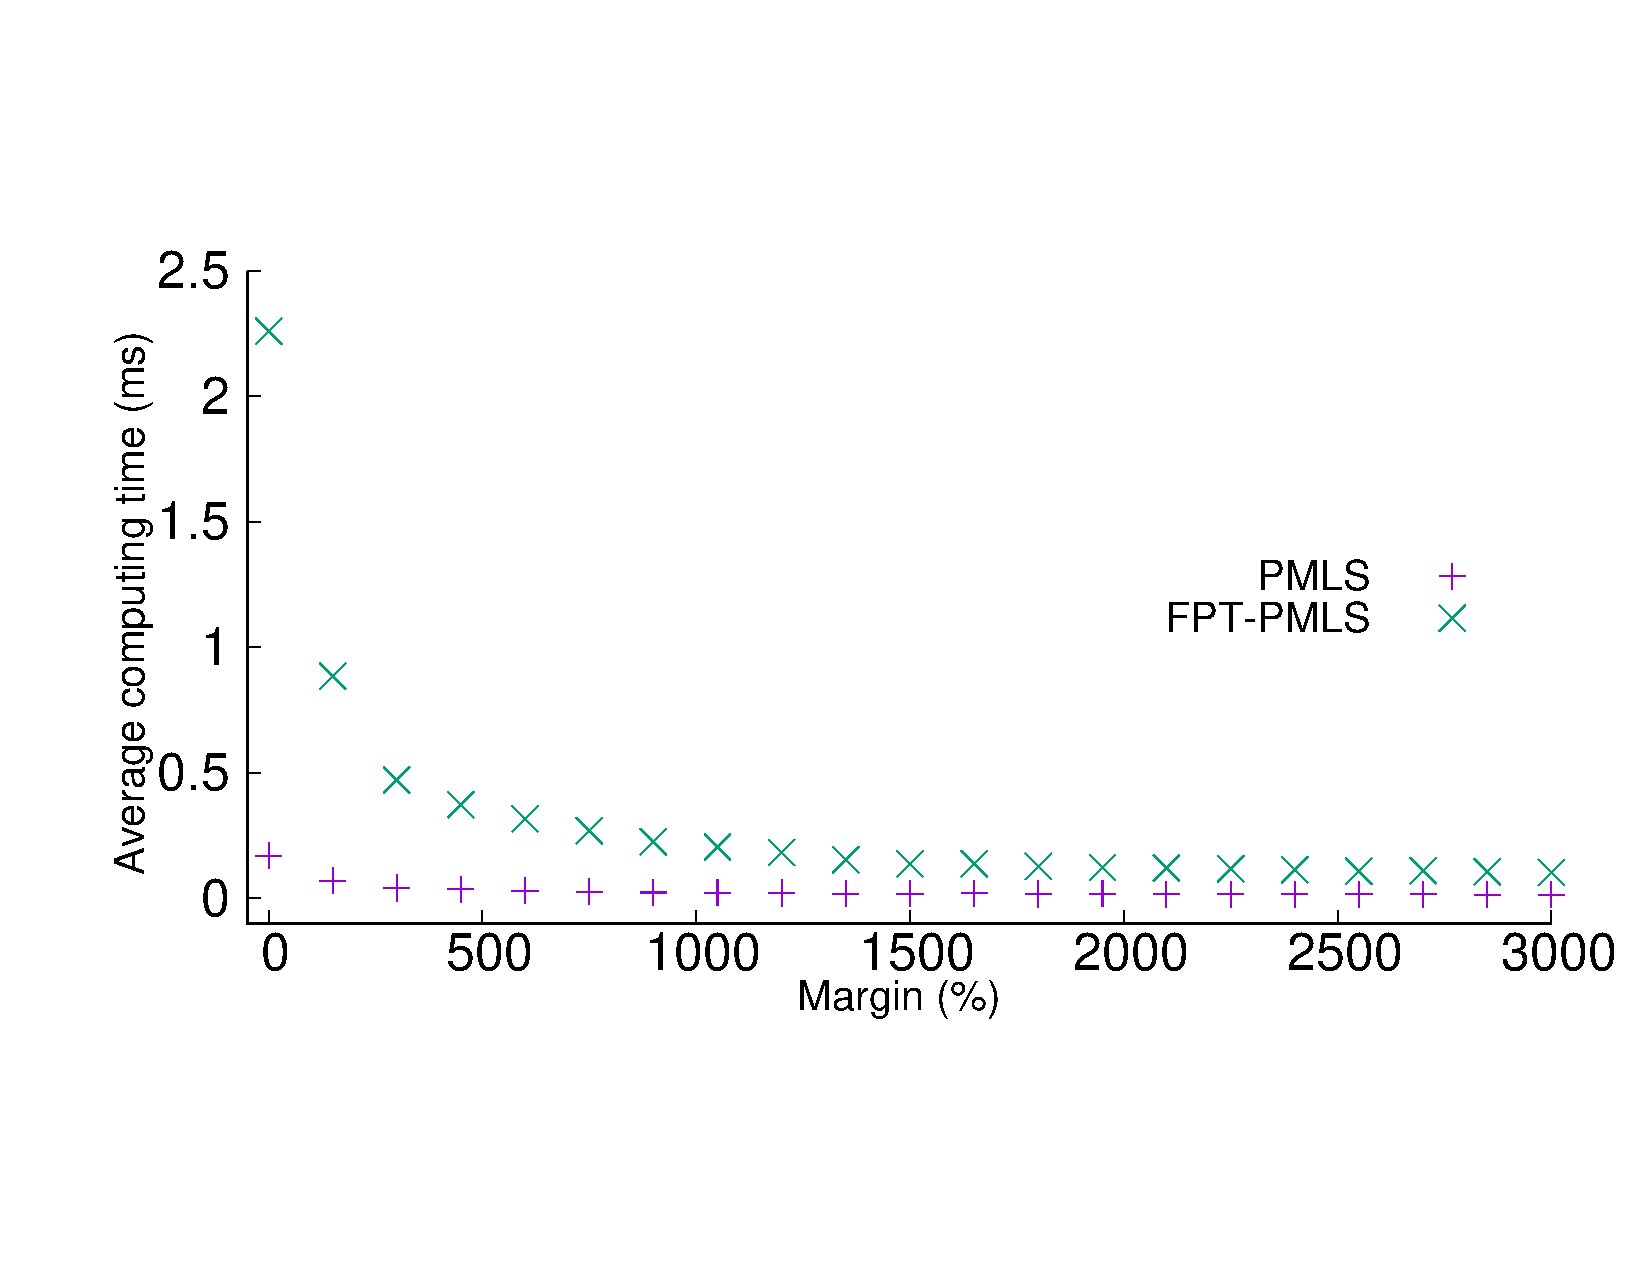
\includegraphics[width=0.5\textwidth]{time_exec.pdf}
%      \end{center}
%      \caption{Computation time of PMLS and FPT-MLS}
%     \label{fig:exec_time}
%     \end{figure}
%
%	First, remark that the computation time of the two algorithm decrease until a margin of approximately  $1,000$ slots. Indeed, the more the algorithm fails, the higher the computation time is because the $1,000$ random orders have to be drawn before failing. Moreover, even when both of the two algorithms always succeed, the computation time of FPT-PMLS is about $10$ time higher that the computation time of the PMLS algorithm. Furthermore, when the FPT-PMLS algorithm could be able to find a solution that the PMLS algorithm would not find, i.e. on low margins, the computation time is $14$ time higher for the first algorithm. It is not really worth it since, most of the time, the FPT-PMLS algorithm do not have a better success rate than the PMLS algorithm.
%     

    When evaluating the computing time of our method, we should take into account how many random orders are drawn. In our experiment, we chose to draw $1,000$ orders which may be 
    $1,000$ time slower than using fixed order. The choice of the number of random orders drawn yields a trade-off between the computation time and the success rate. 
    We investigate the success rate of our algorithms with regards to the number of random orders drawn, a load of $95\%$ and a margin $0$. The table of Figure~\ref{fig:randomdrawing} presents the success rate for each number of sending orders, averaged over $10,000$ instances, for GD, PMLS and FPT-PMLS.
         \begin{figure}[h] 
       \begin{center}
   \begin{tabularx}{0.5\textwidth}{|c|X|X|X|X|X|X|}
    \hline
    \# orders& $1$ & $10$ & $100$& $1,000$& $10^{4}$&$10^{5}$\\
    \hline
    GD & $0.55$ &$6.05$&$35.44$&$77.43$&$90.1$&$92.4$\\
    \hline
  PMLS & $82.04$ &$98.84$&$99.71$&$99.80$&$99.83$&$99.83$\\
    \hline
    FPT-PMLS & $91.33$&$99.17$&$99.72$&$99.80$ &$99.83$&$99.83$\\
    \hline
      \end{tabularx}
      \end{center}
   \caption{Impact of the number of random sending orders}
        \label{fig:randomdrawing}
     \end{figure}

First, observe that the better the algorithm to solve $\bra$, the less random order it needs in stage one to achieve its best performances. In particular, FPT-PMLS has better results than PMLS for less than $1,000$ random orders, but not beyond. This justifies our choice to draw $1,000$ random orders, to obtain the best success rate within the smallest time.

Also, remark that the number of different orders is $7!= 5,040$ since we have $8$ routes and the solutions are invariant up to a circular permutation of the order. Hence for $8$ routes, it is possible to test every possible order. However the computation time of this method scales badly with $n$. The fact that PMLS and FPT-PMLS have already high success rates for $10$ random orders hints that even for larger $n$, drawing $1000$ random orders is sufficient.

%
%
%First, we observe that the FPT-PMLS gives some better results than PMLS for less than $1,000$ random orders, but not beyond. This enforce our choice to draw $1,000$ random orders, to have the same performances with PMLS, which have a better complexity.
%Also, remark that we can improve our previous results by taking $10,000$ random orders,
%instead of $1,000$. The number of different orders is $7!= 5,040$ since we have $8$ routes and the solutions are invariant up to a circular permutation of the order. Therefore instead of doing $10,000$ random draws we could test every possible order in less time. However the computation time of this method would scale badly with $n$. On the other hand, remark that the success rate of PMLS is already high for $100$ random orders, which means it will work even better than the other methods when $n$ is larger and that the number of random orders drawn becomes critical.
%     \subsubsection{Some harder topologies to stress PMLS}
%     The previous results are computed on instances in which the size of the arcs in the network are uniformly drawn. We now want to study the impact of the topology of the network on the performances of PMLS. We remarked that the performances of PMLS are the worst if we draw all the routes in the same range of values. This observation contradict the remarks of the beginning of the section~\ref{sec:PALL}. Indeed, in this remark, we explain that if all the routes are the same or almost the same, the problem \pall is easy to solve in time $O(n)$. Nevertheless, if the routes are drawn in the same range of values, by increasing this range, we move out from the instances which are easy to solve. Figures~\ref{fig:1grp}~and~\ref{fig:2grp} show the impact of the difference between the size of the routes on the efficiency of PMLS. On figure~\ref{fig:1grp}, we draw the all arcs of the network between $P-{\text range}$ and $P$, varying the range from $0$ to $3200$. On figure~\ref{fig:2grp}, we draw half of the arcs between $P-{\text range}$ and $P$, and half of the arcs between $\frac{P}{2}-\text{range}$ and $\frac{P}{2}$. The figures shows the cumulative distribution of the margin needed by PMLS to find a solution, computed on $10,000$ instances.


     \subsubsection{Harder random topologies}
     
     The previous experiments use instances where the weights of the arcs in the network are uniformly drawn in a large interval. However, it is quite natural to consider that most routes are of roughly the same length or can be arranged in two groups of similar lengths if the network involves two data-centers.
     
     By Theorem~\ref{th:asym}, there is an assignment with margin equal to the difference
     between the sizes of the routes. Hence if the routes have all almost the same size, the needed margin is small. Moreover, if the routes are drawn in a large interval, then the expected difference between the longest route and the second longest is large. This difference can be seen as a free latency for all routes, hence we expect to need little margin in this regime too. As a consequence, the harder instances should be for routes with length 
     drawn in an interval of a moderate size compared to the period.
     
     The figures~\ref{fig:1grp} and~\ref{fig:2grp} show the cumulative distribution of the margin needed by PMLS to find an assignment computed on $10,000$ instances.
     Figure~\ref{fig:1grp} represents the success rate of PMLS for instances where length of arcs are drawn in $[P-I,P+I]$, where $I$ goes from $0$ to $3200$. As expected the success rate decreases when the range increases until $I = 800$ and then increases again.  In the the most difficult settings, only $78\%$ of the instances can be solved with margin $0$, and we need a margin of $1,900$ to ensure that PMLS finds a solution.
    
     In Figure~\ref{fig:2grp}, we do the same experiment, except that the weight of arcs of half of the routes is drawn in $[P-I,P+I]$ and the length of the other half is drawn in $[P/2-I,P/2 + I]$. The situation is the same as for the previous experiment but with better success rates. 

          
              \begin{figure}
       \begin{center}
      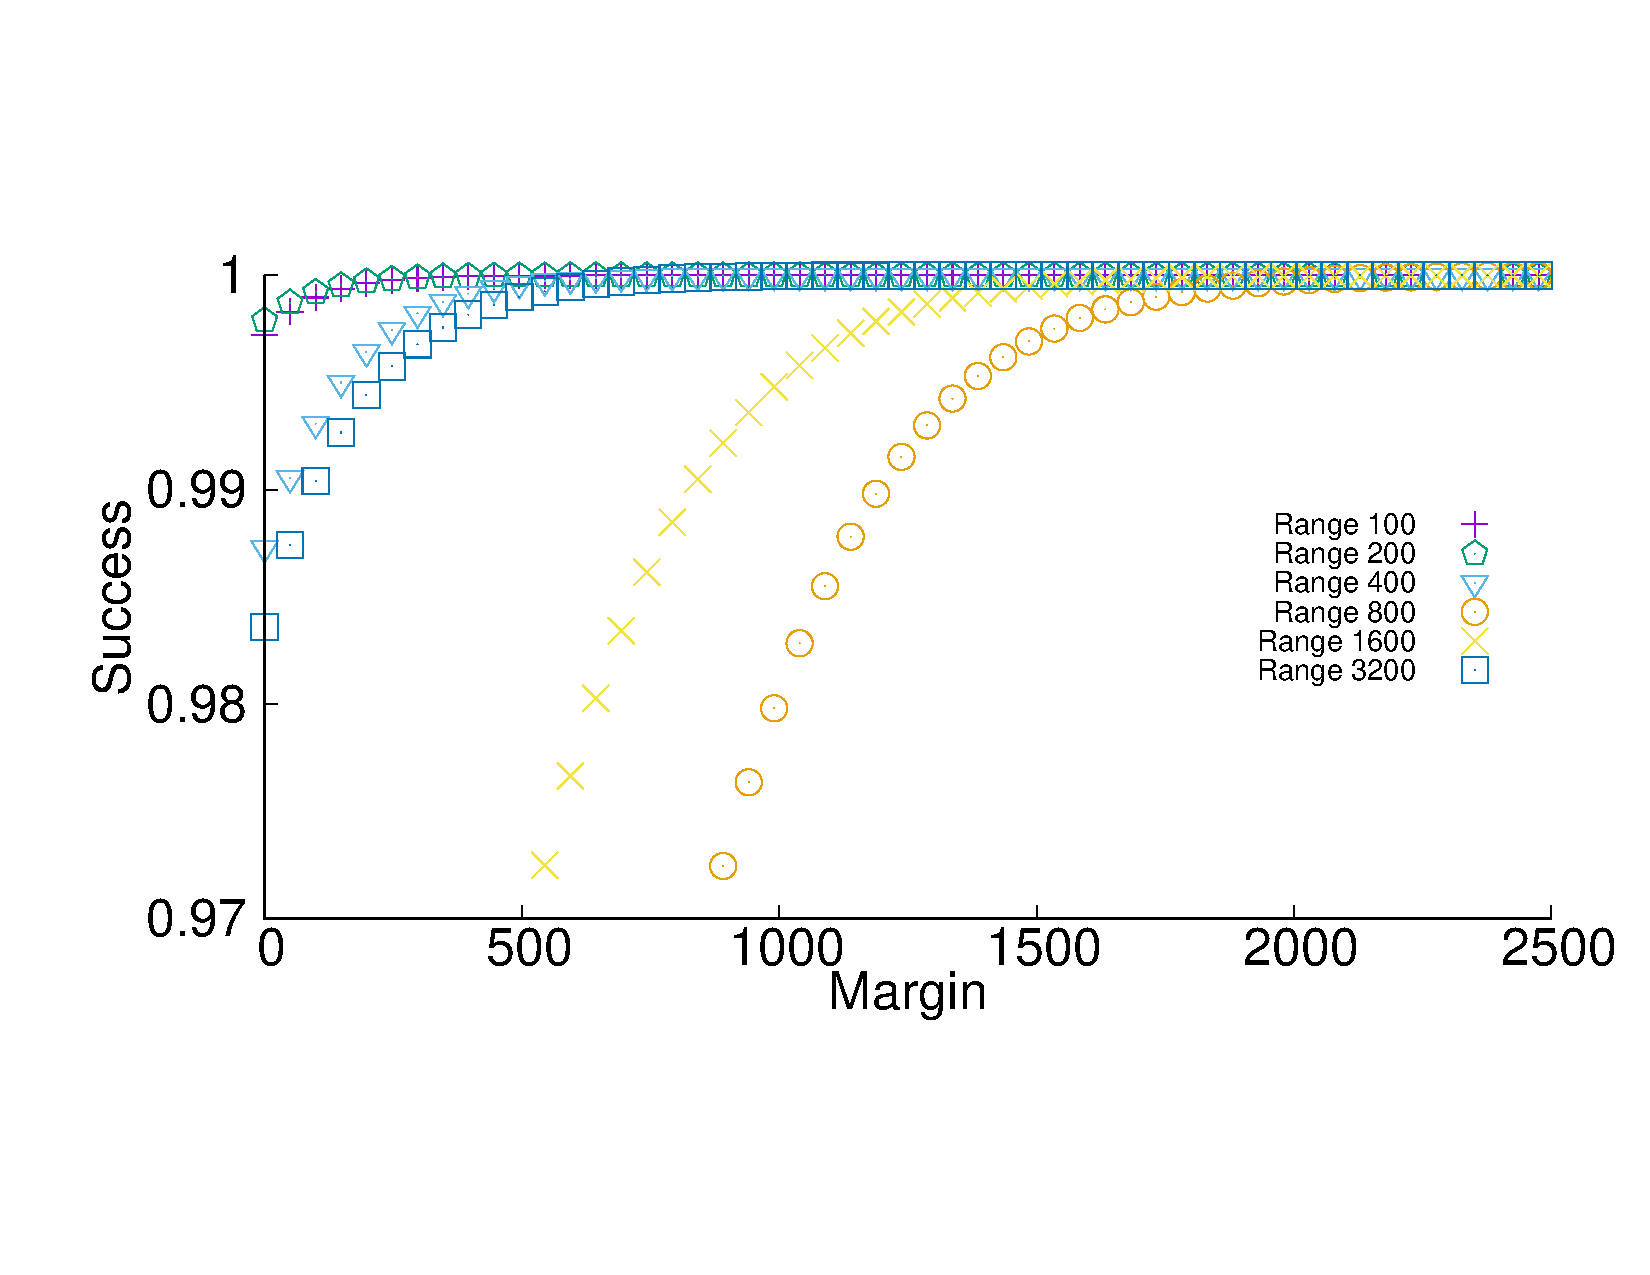
\includegraphics[width = 0.5\textwidth]{departs_distrib1Grp.pdf}
      \end{center}
      \caption{Cumulative distribution of the margin needed to find an assignment}
      \label{fig:1grp}   
     \end{figure}    
     
                \begin{figure}
       \begin{center}
      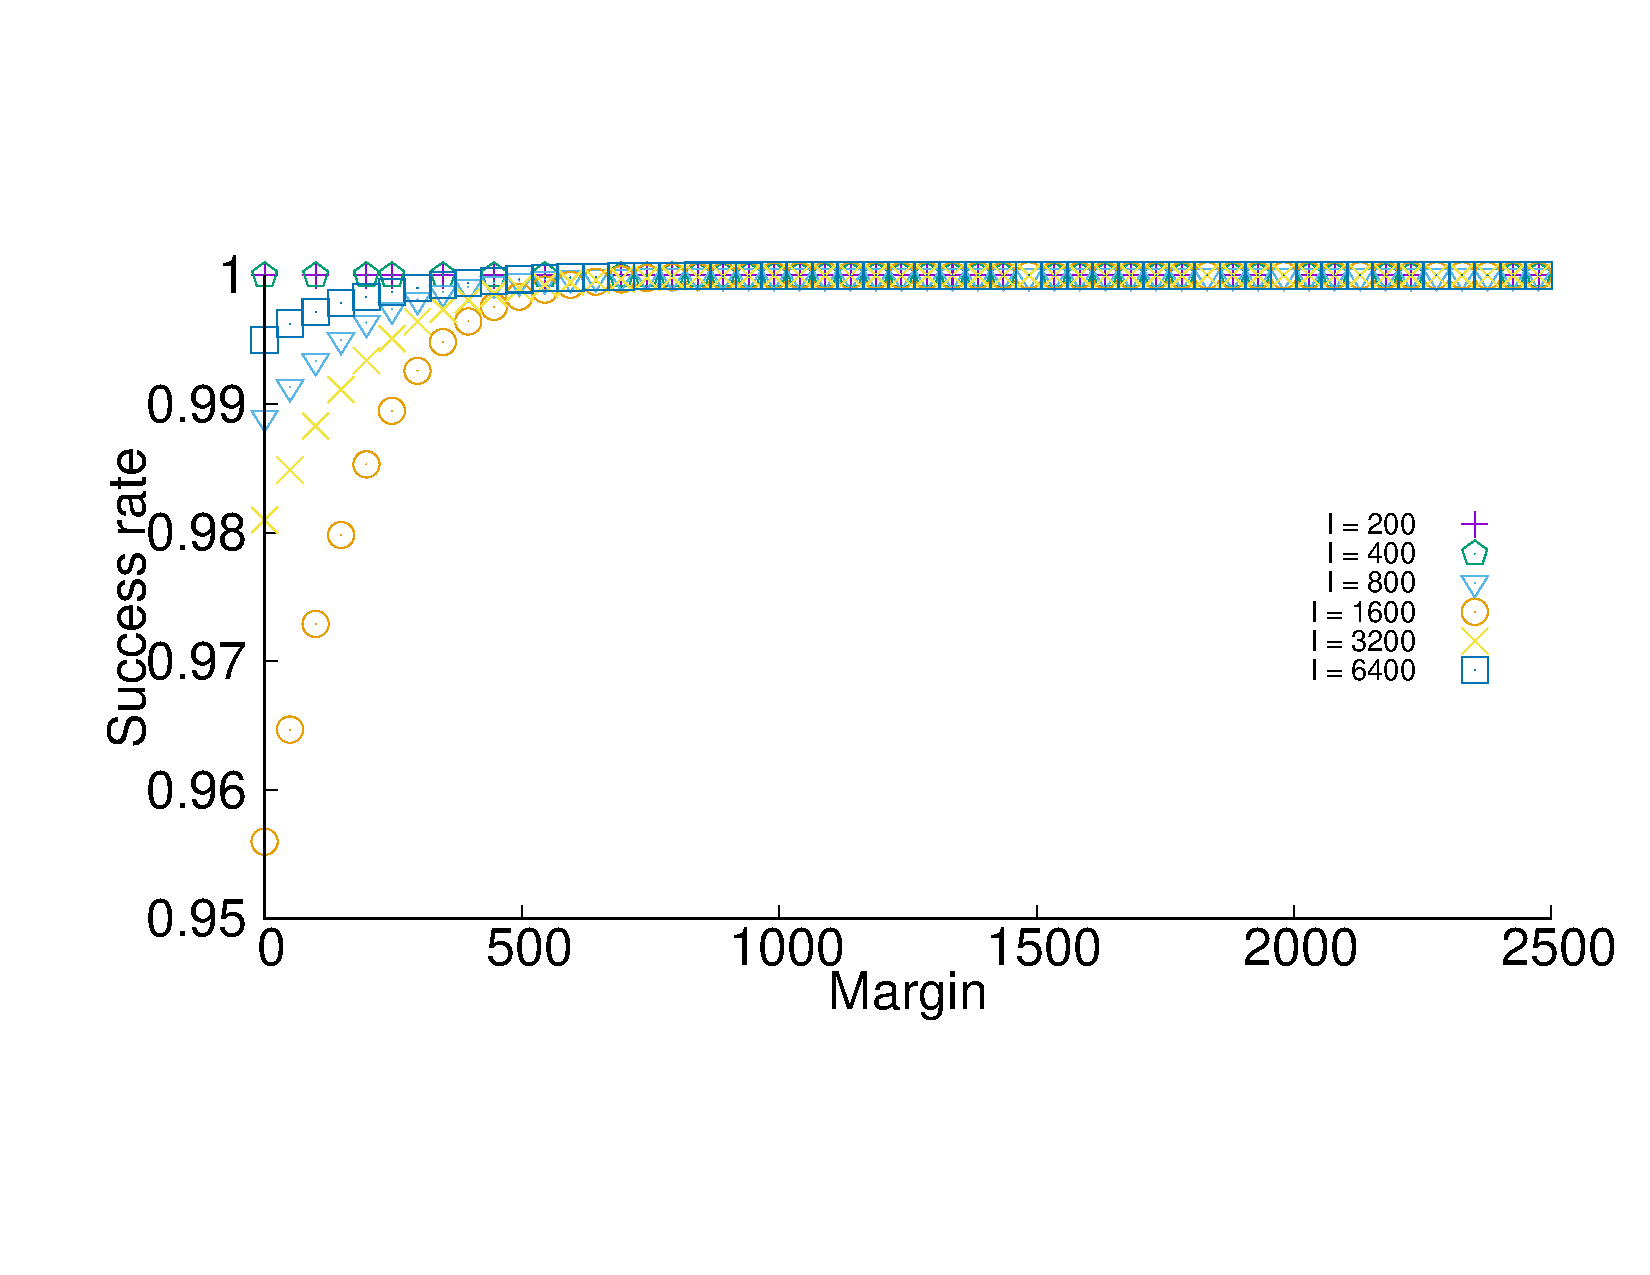
\includegraphics[width = 0.5\textwidth]{departs_distrib2Grp.pdf}
      \end{center}
    \caption{Cumulative distribution of the margin needed to find an assignment with two groups of routes}
      \label{fig:2grp}   
     \end{figure}    
     
     

\section{Periodic sending vs statistical multiplexing}\label{sec:comparison}

     \subsection{Sending schemes produced by PMLS compared to Statistical multiplexing}

     \textbf{TODO:} donner deux politiques de buffering: FIFO, deadline et les comparer à PMLS.


     Now that we have found the best amongst the algorithms solving \pall, we need to compare its performances against the actual way to manage the messages in a network:  statistical multiplexing, with a FIFO buffer in each node of the network to resolve collisions. The time at which the messages are sent in the network is not computed as in our approach, thus we fix the offsets of each route to some random value.
     Even if this policy seems to work in practice when the network is not too loaded, it does not give any guarantee on the latency. Remark that the process is not periodic, therefore we must measure the process time of each route over several periods if we want to compute its maximum. We choose to simulate it for $1,000$ periods and we have observed that the process time usually stabilizes after $10$ periods. The margin is defined as the maximum process time, computed as explained, minus twice the size of the longest route. 
	    
     In Figure~\ref{fig:sto}~and~\ref{fig:stobad}, we represent the probability of success for 
     statistical multiplexing and PMLS for different margins. The success rates are computed from $10,000$ star routed networks for each margin. On Figure~\ref{fig:sto}, the arcs of the network are uniformly drawn between $0$ and $20,000$, while on Figure~\ref{fig:stobad}, the arcs of the network are uniformly drawn between $P-800$ and $P+800$. The others parameters of the experiences are the same as previously. We represent the distribution under high and light load for statistical multiplexing and under high load only for PMLS since under light load the margin is always $0$. 
     

    \begin{figure}
       \begin{center}
      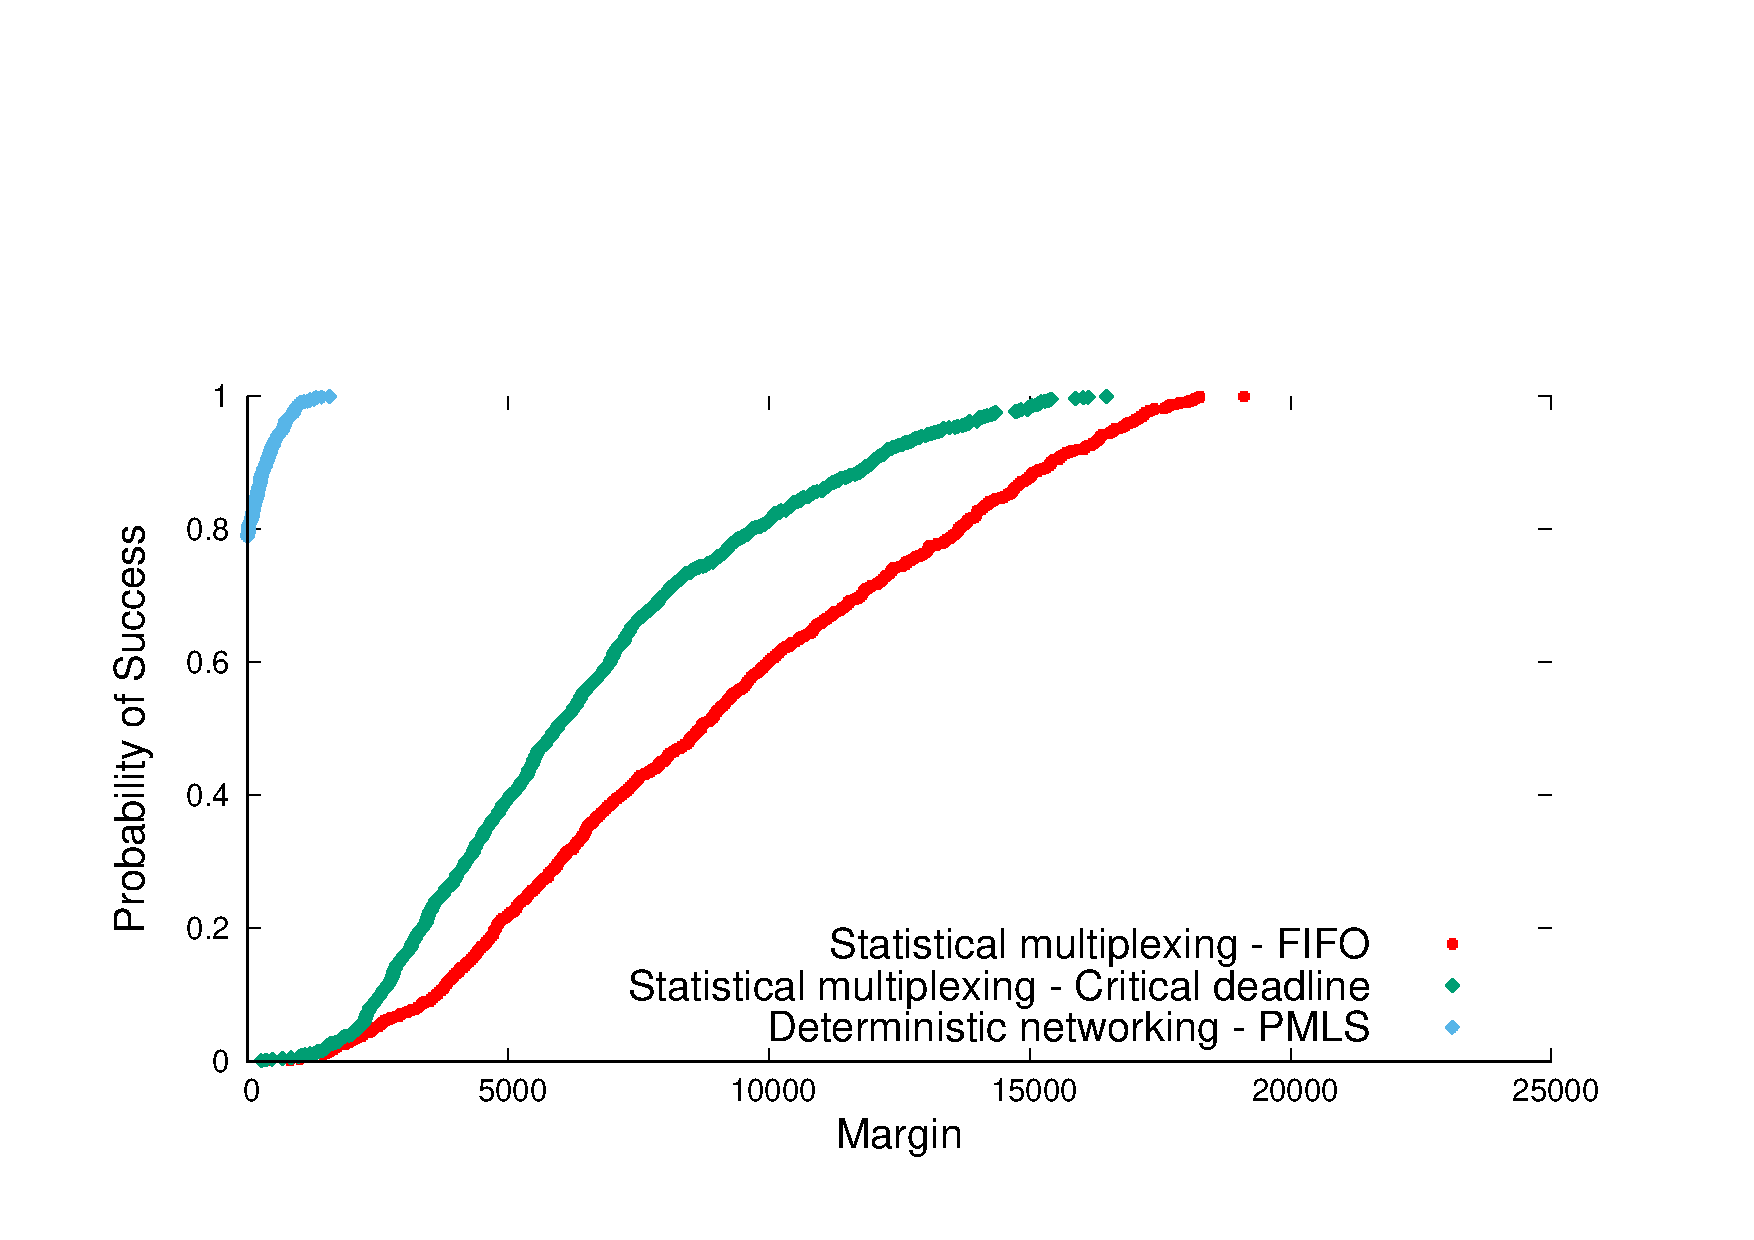
\includegraphics[width = 0.45\textwidth]{stochastic.pdf}
       %% GNUPLOT: LaTeX picture
\setlength{\unitlength}{0.240900pt}
\ifx\plotpoint\undefined\newsavebox{\plotpoint}\fi
\sbox{\plotpoint}{\rule[-0.200pt]{0.400pt}{0.400pt}}%
\begin{picture}(1500,900)(0,0)
\sbox{\plotpoint}{\rule[-0.200pt]{0.400pt}{0.400pt}}%
\put(171.0,131.0){\rule[-0.200pt]{4.818pt}{0.400pt}}
\put(151,131){\makebox(0,0)[r]{$0$}}
\put(1279.0,131.0){\rule[-0.200pt]{4.818pt}{0.400pt}}
\put(171.0,212.0){\rule[-0.200pt]{4.818pt}{0.400pt}}
\put(151,212){\makebox(0,0)[r]{$1000$}}
\put(1279.0,212.0){\rule[-0.200pt]{4.818pt}{0.400pt}}
\put(171.0,293.0){\rule[-0.200pt]{4.818pt}{0.400pt}}
\put(151,293){\makebox(0,0)[r]{$2000$}}
\put(1279.0,293.0){\rule[-0.200pt]{4.818pt}{0.400pt}}
\put(171.0,374.0){\rule[-0.200pt]{4.818pt}{0.400pt}}
\put(151,374){\makebox(0,0)[r]{$3000$}}
\put(1279.0,374.0){\rule[-0.200pt]{4.818pt}{0.400pt}}
\put(171.0,455.0){\rule[-0.200pt]{4.818pt}{0.400pt}}
\put(151,455){\makebox(0,0)[r]{$4000$}}
\put(1279.0,455.0){\rule[-0.200pt]{4.818pt}{0.400pt}}
\put(171.0,535.0){\rule[-0.200pt]{4.818pt}{0.400pt}}
\put(151,535){\makebox(0,0)[r]{$5000$}}
\put(1279.0,535.0){\rule[-0.200pt]{4.818pt}{0.400pt}}
\put(171.0,616.0){\rule[-0.200pt]{4.818pt}{0.400pt}}
\put(151,616){\makebox(0,0)[r]{$6000$}}
\put(1279.0,616.0){\rule[-0.200pt]{4.818pt}{0.400pt}}
\put(171.0,697.0){\rule[-0.200pt]{4.818pt}{0.400pt}}
\put(151,697){\makebox(0,0)[r]{$7000$}}
\put(1279.0,697.0){\rule[-0.200pt]{4.818pt}{0.400pt}}
\put(171.0,778.0){\rule[-0.200pt]{4.818pt}{0.400pt}}
\put(151,778){\makebox(0,0)[r]{$8000$}}
\put(1279.0,778.0){\rule[-0.200pt]{4.818pt}{0.400pt}}
\put(171.0,859.0){\rule[-0.200pt]{4.818pt}{0.400pt}}
\put(151,859){\makebox(0,0)[r]{$9000$}}
\put(1279.0,859.0){\rule[-0.200pt]{4.818pt}{0.400pt}}
\put(171.0,131.0){\rule[-0.200pt]{0.400pt}{4.818pt}}
\put(171,90){\makebox(0,0){$20000$}}
\put(171.0,839.0){\rule[-0.200pt]{0.400pt}{4.818pt}}
\put(359.0,131.0){\rule[-0.200pt]{0.400pt}{4.818pt}}
\put(359,90){\makebox(0,0){$25000$}}
\put(359.0,839.0){\rule[-0.200pt]{0.400pt}{4.818pt}}
\put(547.0,131.0){\rule[-0.200pt]{0.400pt}{4.818pt}}
\put(547,90){\makebox(0,0){$30000$}}
\put(547.0,839.0){\rule[-0.200pt]{0.400pt}{4.818pt}}
\put(735.0,131.0){\rule[-0.200pt]{0.400pt}{4.818pt}}
\put(735,90){\makebox(0,0){$35000$}}
\put(735.0,839.0){\rule[-0.200pt]{0.400pt}{4.818pt}}
\put(923.0,131.0){\rule[-0.200pt]{0.400pt}{4.818pt}}
\put(923,90){\makebox(0,0){$40000$}}
\put(923.0,839.0){\rule[-0.200pt]{0.400pt}{4.818pt}}
\put(1111.0,131.0){\rule[-0.200pt]{0.400pt}{4.818pt}}
\put(1111,90){\makebox(0,0){$45000$}}
\put(1111.0,839.0){\rule[-0.200pt]{0.400pt}{4.818pt}}
\put(1299.0,131.0){\rule[-0.200pt]{0.400pt}{4.818pt}}
\put(1299,90){\makebox(0,0){$50000$}}
\put(1299.0,839.0){\rule[-0.200pt]{0.400pt}{4.818pt}}
\put(171.0,131.0){\rule[-0.200pt]{0.400pt}{175.375pt}}
\put(171.0,131.0){\rule[-0.200pt]{271.735pt}{0.400pt}}
\put(30,495){\makebox(0,0){Needed Flexibility}}
\put(735,29){\makebox(0,0){Period}}
\put(171.0,455.0){\rule[-0.200pt]{0.400pt}{81.183pt}}
\put(171.0,455.0){\rule[-0.200pt]{2.409pt}{0.400pt}}
\put(171.0,792.0){\rule[-0.200pt]{2.409pt}{0.400pt}}
\put(209.0,412.0){\rule[-0.200pt]{0.400pt}{73.715pt}}
\put(199.0,412.0){\rule[-0.200pt]{4.818pt}{0.400pt}}
\put(199.0,718.0){\rule[-0.200pt]{4.818pt}{0.400pt}}
\put(246.0,353.0){\rule[-0.200pt]{0.400pt}{79.497pt}}
\put(236.0,353.0){\rule[-0.200pt]{4.818pt}{0.400pt}}
\put(236.0,683.0){\rule[-0.200pt]{4.818pt}{0.400pt}}
\put(284.0,336.0){\rule[-0.200pt]{0.400pt}{75.883pt}}
\put(274.0,336.0){\rule[-0.200pt]{4.818pt}{0.400pt}}
\put(274.0,651.0){\rule[-0.200pt]{4.818pt}{0.400pt}}
\put(321.0,306.0){\rule[-0.200pt]{0.400pt}{70.343pt}}
\put(311.0,306.0){\rule[-0.200pt]{4.818pt}{0.400pt}}
\put(311.0,598.0){\rule[-0.200pt]{4.818pt}{0.400pt}}
\put(359.0,297.0){\rule[-0.200pt]{0.400pt}{73.715pt}}
\put(349.0,297.0){\rule[-0.200pt]{4.818pt}{0.400pt}}
\put(349.0,603.0){\rule[-0.200pt]{4.818pt}{0.400pt}}
\put(397.0,270.0){\rule[-0.200pt]{0.400pt}{63.598pt}}
\put(387.0,270.0){\rule[-0.200pt]{4.818pt}{0.400pt}}
\put(387.0,534.0){\rule[-0.200pt]{4.818pt}{0.400pt}}
\put(434.0,269.0){\rule[-0.200pt]{0.400pt}{64.561pt}}
\put(424.0,269.0){\rule[-0.200pt]{4.818pt}{0.400pt}}
\put(424.0,537.0){\rule[-0.200pt]{4.818pt}{0.400pt}}
\put(472.0,238.0){\rule[-0.200pt]{0.400pt}{69.138pt}}
\put(462.0,238.0){\rule[-0.200pt]{4.818pt}{0.400pt}}
\put(462.0,525.0){\rule[-0.200pt]{4.818pt}{0.400pt}}
\put(509.0,226.0){\rule[-0.200pt]{0.400pt}{62.393pt}}
\put(499.0,226.0){\rule[-0.200pt]{4.818pt}{0.400pt}}
\put(499.0,485.0){\rule[-0.200pt]{4.818pt}{0.400pt}}
\put(547.0,222.0){\rule[-0.200pt]{0.400pt}{60.225pt}}
\put(537.0,222.0){\rule[-0.200pt]{4.818pt}{0.400pt}}
\put(537.0,472.0){\rule[-0.200pt]{4.818pt}{0.400pt}}
\put(585.0,195.0){\rule[-0.200pt]{0.400pt}{60.225pt}}
\put(575.0,195.0){\rule[-0.200pt]{4.818pt}{0.400pt}}
\put(575.0,445.0){\rule[-0.200pt]{4.818pt}{0.400pt}}
\put(622.0,185.0){\rule[-0.200pt]{0.400pt}{58.780pt}}
\put(612.0,185.0){\rule[-0.200pt]{4.818pt}{0.400pt}}
\put(612.0,429.0){\rule[-0.200pt]{4.818pt}{0.400pt}}
\put(660.0,178.0){\rule[-0.200pt]{0.400pt}{59.743pt}}
\put(650.0,178.0){\rule[-0.200pt]{4.818pt}{0.400pt}}
\put(650.0,426.0){\rule[-0.200pt]{4.818pt}{0.400pt}}
\put(697.0,188.0){\rule[-0.200pt]{0.400pt}{59.020pt}}
\put(687.0,188.0){\rule[-0.200pt]{4.818pt}{0.400pt}}
\put(687.0,433.0){\rule[-0.200pt]{4.818pt}{0.400pt}}
\put(735.0,152.0){\rule[-0.200pt]{0.400pt}{55.889pt}}
\put(725.0,152.0){\rule[-0.200pt]{4.818pt}{0.400pt}}
\put(725.0,384.0){\rule[-0.200pt]{4.818pt}{0.400pt}}
\put(773.0,146.0){\rule[-0.200pt]{0.400pt}{57.575pt}}
\put(763.0,146.0){\rule[-0.200pt]{4.818pt}{0.400pt}}
\put(763.0,385.0){\rule[-0.200pt]{4.818pt}{0.400pt}}
\put(810.0,146.0){\rule[-0.200pt]{0.400pt}{54.925pt}}
\put(800.0,146.0){\rule[-0.200pt]{4.818pt}{0.400pt}}
\put(800.0,374.0){\rule[-0.200pt]{4.818pt}{0.400pt}}
\put(848.0,143.0){\rule[-0.200pt]{0.400pt}{56.371pt}}
\put(838.0,143.0){\rule[-0.200pt]{4.818pt}{0.400pt}}
\put(838.0,377.0){\rule[-0.200pt]{4.818pt}{0.400pt}}
\put(885.0,140.0){\rule[-0.200pt]{0.400pt}{56.371pt}}
\put(875.0,140.0){\rule[-0.200pt]{4.818pt}{0.400pt}}
\put(875.0,374.0){\rule[-0.200pt]{4.818pt}{0.400pt}}
\put(923.0,133.0){\rule[-0.200pt]{0.400pt}{54.202pt}}
\put(913.0,133.0){\rule[-0.200pt]{4.818pt}{0.400pt}}
\put(913.0,358.0){\rule[-0.200pt]{4.818pt}{0.400pt}}
\put(961.0,131.0){\rule[-0.200pt]{0.400pt}{55.166pt}}
\put(951.0,131.0){\rule[-0.200pt]{4.818pt}{0.400pt}}
\put(951.0,360.0){\rule[-0.200pt]{4.818pt}{0.400pt}}
\put(998.0,131.0){\rule[-0.200pt]{0.400pt}{49.384pt}}
\put(988.0,131.0){\rule[-0.200pt]{4.818pt}{0.400pt}}
\put(988.0,336.0){\rule[-0.200pt]{4.818pt}{0.400pt}}
\put(1036.0,131.0){\rule[-0.200pt]{0.400pt}{48.180pt}}
\put(1026.0,131.0){\rule[-0.200pt]{4.818pt}{0.400pt}}
\put(1026.0,331.0){\rule[-0.200pt]{4.818pt}{0.400pt}}
\put(1073.0,131.0){\rule[-0.200pt]{0.400pt}{47.216pt}}
\put(1063.0,131.0){\rule[-0.200pt]{4.818pt}{0.400pt}}
\put(1063.0,327.0){\rule[-0.200pt]{4.818pt}{0.400pt}}
\put(1111.0,131.0){\rule[-0.200pt]{0.400pt}{46.975pt}}
\put(1101.0,131.0){\rule[-0.200pt]{4.818pt}{0.400pt}}
\put(1101.0,326.0){\rule[-0.200pt]{4.818pt}{0.400pt}}
\put(1149.0,131.0){\rule[-0.200pt]{0.400pt}{45.048pt}}
\put(1139.0,131.0){\rule[-0.200pt]{4.818pt}{0.400pt}}
\put(1139.0,318.0){\rule[-0.200pt]{4.818pt}{0.400pt}}
\put(1186.0,131.0){\rule[-0.200pt]{0.400pt}{46.494pt}}
\put(1176.0,131.0){\rule[-0.200pt]{4.818pt}{0.400pt}}
\put(1176.0,324.0){\rule[-0.200pt]{4.818pt}{0.400pt}}
\put(1224.0,131.0){\rule[-0.200pt]{0.400pt}{45.048pt}}
\put(1214.0,131.0){\rule[-0.200pt]{4.818pt}{0.400pt}}
\put(1214.0,318.0){\rule[-0.200pt]{4.818pt}{0.400pt}}
\put(1261.0,131.0){\rule[-0.200pt]{0.400pt}{41.194pt}}
\put(1251.0,131.0){\rule[-0.200pt]{4.818pt}{0.400pt}}
\put(171,608){\makebox(0,0){$+$}}
\put(209,562){\makebox(0,0){$+$}}
\put(246,503){\makebox(0,0){$+$}}
\put(284,479){\makebox(0,0){$+$}}
\put(321,431){\makebox(0,0){$+$}}
\put(359,429){\makebox(0,0){$+$}}
\put(397,390){\makebox(0,0){$+$}}
\put(434,382){\makebox(0,0){$+$}}
\put(472,367){\makebox(0,0){$+$}}
\put(509,340){\makebox(0,0){$+$}}
\put(547,327){\makebox(0,0){$+$}}
\put(585,317){\makebox(0,0){$+$}}
\put(622,307){\makebox(0,0){$+$}}
\put(660,302){\makebox(0,0){$+$}}
\put(697,300){\makebox(0,0){$+$}}
\put(735,278){\makebox(0,0){$+$}}
\put(773,273){\makebox(0,0){$+$}}
\put(810,268){\makebox(0,0){$+$}}
\put(848,267){\makebox(0,0){$+$}}
\put(885,254){\makebox(0,0){$+$}}
\put(923,248){\makebox(0,0){$+$}}
\put(961,259){\makebox(0,0){$+$}}
\put(998,234){\makebox(0,0){$+$}}
\put(1036,234){\makebox(0,0){$+$}}
\put(1073,232){\makebox(0,0){$+$}}
\put(1111,228){\makebox(0,0){$+$}}
\put(1149,216){\makebox(0,0){$+$}}
\put(1186,212){\makebox(0,0){$+$}}
\put(1224,227){\makebox(0,0){$+$}}
\put(1261,203){\makebox(0,0){$+$}}
\put(1251.0,302.0){\rule[-0.200pt]{4.818pt}{0.400pt}}
\put(171.0,131.0){\rule[-0.200pt]{0.400pt}{175.375pt}}
\put(171.0,131.0){\rule[-0.200pt]{271.735pt}{0.400pt}}
\end{picture}

      \end{center}
      \caption{Probability of success of statistical multiplexing and PMLS for several margins on random topologies}
      \label{fig:sto}   
     \end{figure}    
     
         \begin{figure}
       \begin{center}
      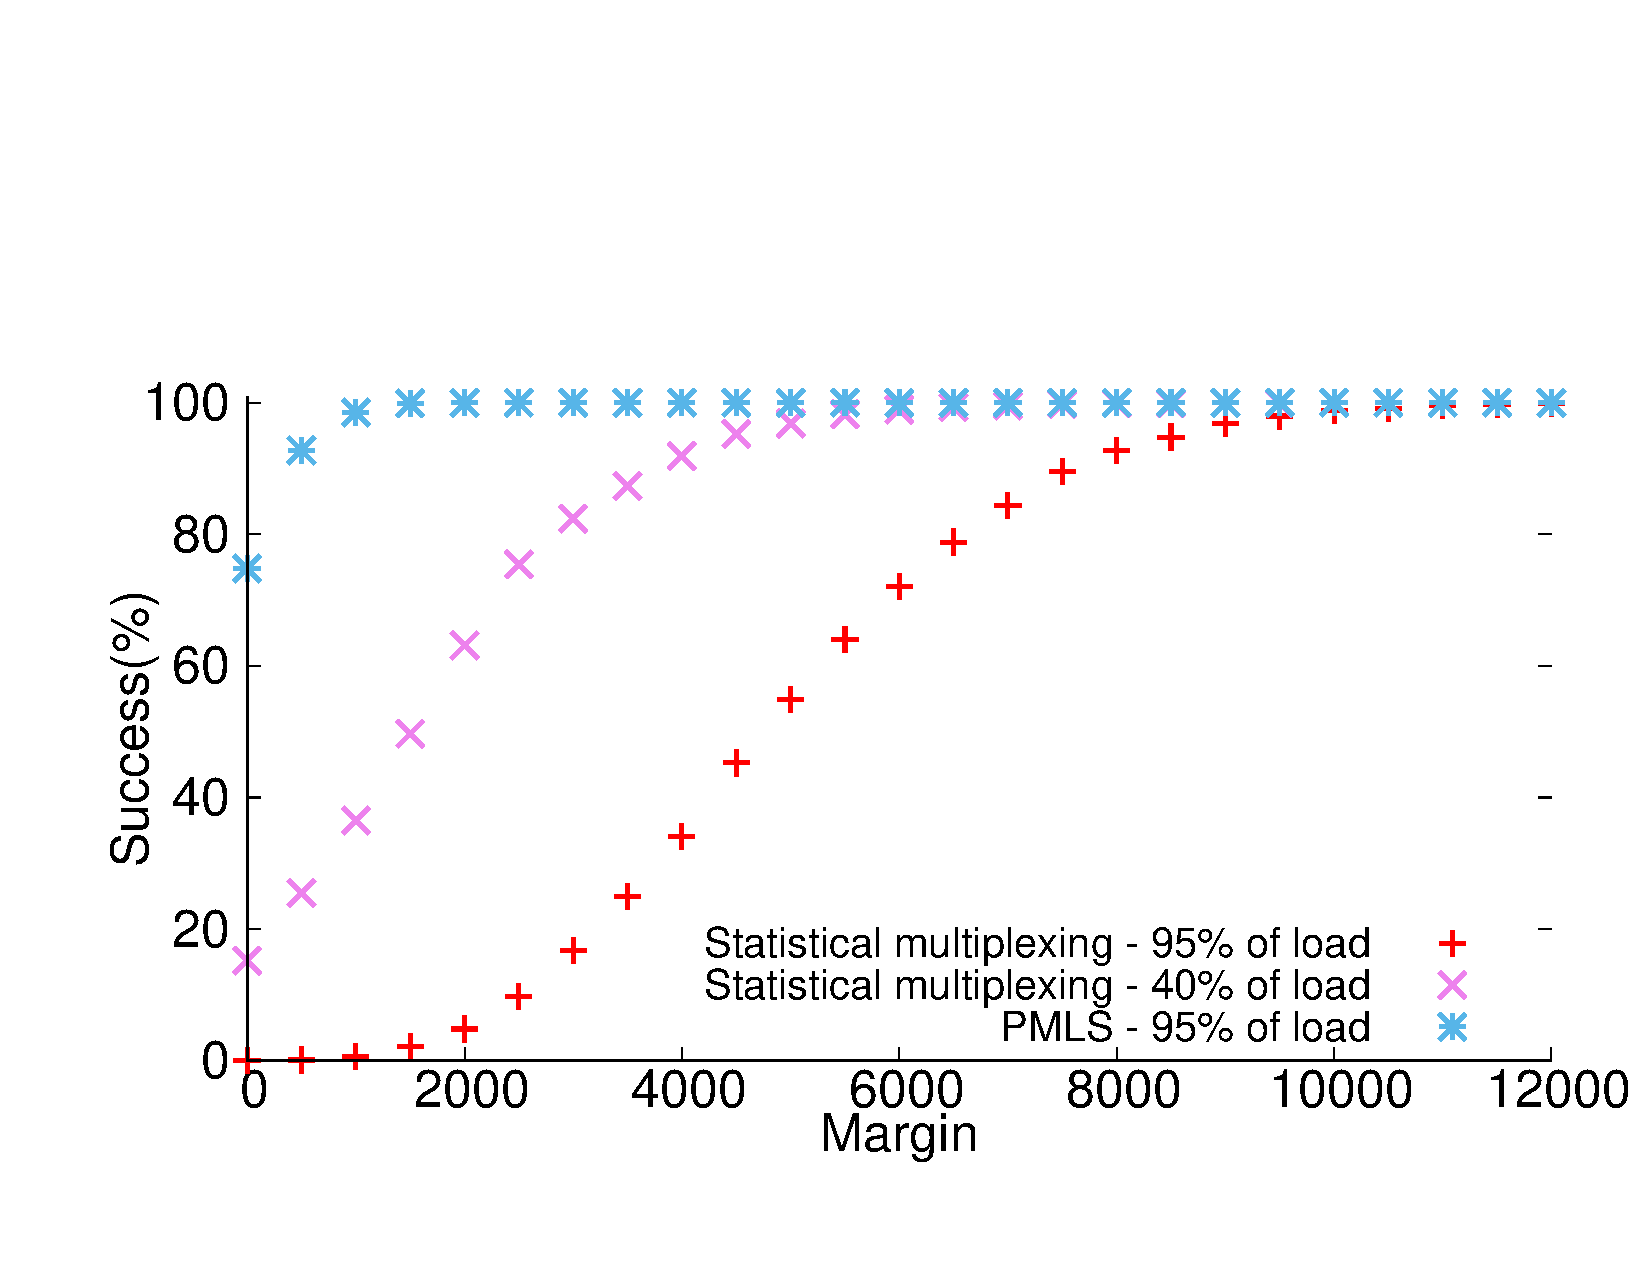
\includegraphics[width = 0.45\textwidth]{stochasticbad.pdf}
       %% GNUPLOT: LaTeX picture
\setlength{\unitlength}{0.240900pt}
\ifx\plotpoint\undefined\newsavebox{\plotpoint}\fi
\sbox{\plotpoint}{\rule[-0.200pt]{0.400pt}{0.400pt}}%
\begin{picture}(1500,900)(0,0)
\sbox{\plotpoint}{\rule[-0.200pt]{0.400pt}{0.400pt}}%
\put(171.0,131.0){\rule[-0.200pt]{4.818pt}{0.400pt}}
\put(151,131){\makebox(0,0)[r]{$0$}}
\put(1279.0,131.0){\rule[-0.200pt]{4.818pt}{0.400pt}}
\put(171.0,212.0){\rule[-0.200pt]{4.818pt}{0.400pt}}
\put(151,212){\makebox(0,0)[r]{$1000$}}
\put(1279.0,212.0){\rule[-0.200pt]{4.818pt}{0.400pt}}
\put(171.0,293.0){\rule[-0.200pt]{4.818pt}{0.400pt}}
\put(151,293){\makebox(0,0)[r]{$2000$}}
\put(1279.0,293.0){\rule[-0.200pt]{4.818pt}{0.400pt}}
\put(171.0,374.0){\rule[-0.200pt]{4.818pt}{0.400pt}}
\put(151,374){\makebox(0,0)[r]{$3000$}}
\put(1279.0,374.0){\rule[-0.200pt]{4.818pt}{0.400pt}}
\put(171.0,455.0){\rule[-0.200pt]{4.818pt}{0.400pt}}
\put(151,455){\makebox(0,0)[r]{$4000$}}
\put(1279.0,455.0){\rule[-0.200pt]{4.818pt}{0.400pt}}
\put(171.0,535.0){\rule[-0.200pt]{4.818pt}{0.400pt}}
\put(151,535){\makebox(0,0)[r]{$5000$}}
\put(1279.0,535.0){\rule[-0.200pt]{4.818pt}{0.400pt}}
\put(171.0,616.0){\rule[-0.200pt]{4.818pt}{0.400pt}}
\put(151,616){\makebox(0,0)[r]{$6000$}}
\put(1279.0,616.0){\rule[-0.200pt]{4.818pt}{0.400pt}}
\put(171.0,697.0){\rule[-0.200pt]{4.818pt}{0.400pt}}
\put(151,697){\makebox(0,0)[r]{$7000$}}
\put(1279.0,697.0){\rule[-0.200pt]{4.818pt}{0.400pt}}
\put(171.0,778.0){\rule[-0.200pt]{4.818pt}{0.400pt}}
\put(151,778){\makebox(0,0)[r]{$8000$}}
\put(1279.0,778.0){\rule[-0.200pt]{4.818pt}{0.400pt}}
\put(171.0,859.0){\rule[-0.200pt]{4.818pt}{0.400pt}}
\put(151,859){\makebox(0,0)[r]{$9000$}}
\put(1279.0,859.0){\rule[-0.200pt]{4.818pt}{0.400pt}}
\put(171.0,131.0){\rule[-0.200pt]{0.400pt}{4.818pt}}
\put(171,90){\makebox(0,0){$20000$}}
\put(171.0,839.0){\rule[-0.200pt]{0.400pt}{4.818pt}}
\put(359.0,131.0){\rule[-0.200pt]{0.400pt}{4.818pt}}
\put(359,90){\makebox(0,0){$25000$}}
\put(359.0,839.0){\rule[-0.200pt]{0.400pt}{4.818pt}}
\put(547.0,131.0){\rule[-0.200pt]{0.400pt}{4.818pt}}
\put(547,90){\makebox(0,0){$30000$}}
\put(547.0,839.0){\rule[-0.200pt]{0.400pt}{4.818pt}}
\put(735.0,131.0){\rule[-0.200pt]{0.400pt}{4.818pt}}
\put(735,90){\makebox(0,0){$35000$}}
\put(735.0,839.0){\rule[-0.200pt]{0.400pt}{4.818pt}}
\put(923.0,131.0){\rule[-0.200pt]{0.400pt}{4.818pt}}
\put(923,90){\makebox(0,0){$40000$}}
\put(923.0,839.0){\rule[-0.200pt]{0.400pt}{4.818pt}}
\put(1111.0,131.0){\rule[-0.200pt]{0.400pt}{4.818pt}}
\put(1111,90){\makebox(0,0){$45000$}}
\put(1111.0,839.0){\rule[-0.200pt]{0.400pt}{4.818pt}}
\put(1299.0,131.0){\rule[-0.200pt]{0.400pt}{4.818pt}}
\put(1299,90){\makebox(0,0){$50000$}}
\put(1299.0,839.0){\rule[-0.200pt]{0.400pt}{4.818pt}}
\put(171.0,131.0){\rule[-0.200pt]{0.400pt}{175.375pt}}
\put(171.0,131.0){\rule[-0.200pt]{271.735pt}{0.400pt}}
\put(30,495){\makebox(0,0){Needed Flexibility}}
\put(735,29){\makebox(0,0){Period}}
\put(171.0,455.0){\rule[-0.200pt]{0.400pt}{81.183pt}}
\put(171.0,455.0){\rule[-0.200pt]{2.409pt}{0.400pt}}
\put(171.0,792.0){\rule[-0.200pt]{2.409pt}{0.400pt}}
\put(209.0,412.0){\rule[-0.200pt]{0.400pt}{73.715pt}}
\put(199.0,412.0){\rule[-0.200pt]{4.818pt}{0.400pt}}
\put(199.0,718.0){\rule[-0.200pt]{4.818pt}{0.400pt}}
\put(246.0,353.0){\rule[-0.200pt]{0.400pt}{79.497pt}}
\put(236.0,353.0){\rule[-0.200pt]{4.818pt}{0.400pt}}
\put(236.0,683.0){\rule[-0.200pt]{4.818pt}{0.400pt}}
\put(284.0,336.0){\rule[-0.200pt]{0.400pt}{75.883pt}}
\put(274.0,336.0){\rule[-0.200pt]{4.818pt}{0.400pt}}
\put(274.0,651.0){\rule[-0.200pt]{4.818pt}{0.400pt}}
\put(321.0,306.0){\rule[-0.200pt]{0.400pt}{70.343pt}}
\put(311.0,306.0){\rule[-0.200pt]{4.818pt}{0.400pt}}
\put(311.0,598.0){\rule[-0.200pt]{4.818pt}{0.400pt}}
\put(359.0,297.0){\rule[-0.200pt]{0.400pt}{73.715pt}}
\put(349.0,297.0){\rule[-0.200pt]{4.818pt}{0.400pt}}
\put(349.0,603.0){\rule[-0.200pt]{4.818pt}{0.400pt}}
\put(397.0,270.0){\rule[-0.200pt]{0.400pt}{63.598pt}}
\put(387.0,270.0){\rule[-0.200pt]{4.818pt}{0.400pt}}
\put(387.0,534.0){\rule[-0.200pt]{4.818pt}{0.400pt}}
\put(434.0,269.0){\rule[-0.200pt]{0.400pt}{64.561pt}}
\put(424.0,269.0){\rule[-0.200pt]{4.818pt}{0.400pt}}
\put(424.0,537.0){\rule[-0.200pt]{4.818pt}{0.400pt}}
\put(472.0,238.0){\rule[-0.200pt]{0.400pt}{69.138pt}}
\put(462.0,238.0){\rule[-0.200pt]{4.818pt}{0.400pt}}
\put(462.0,525.0){\rule[-0.200pt]{4.818pt}{0.400pt}}
\put(509.0,226.0){\rule[-0.200pt]{0.400pt}{62.393pt}}
\put(499.0,226.0){\rule[-0.200pt]{4.818pt}{0.400pt}}
\put(499.0,485.0){\rule[-0.200pt]{4.818pt}{0.400pt}}
\put(547.0,222.0){\rule[-0.200pt]{0.400pt}{60.225pt}}
\put(537.0,222.0){\rule[-0.200pt]{4.818pt}{0.400pt}}
\put(537.0,472.0){\rule[-0.200pt]{4.818pt}{0.400pt}}
\put(585.0,195.0){\rule[-0.200pt]{0.400pt}{60.225pt}}
\put(575.0,195.0){\rule[-0.200pt]{4.818pt}{0.400pt}}
\put(575.0,445.0){\rule[-0.200pt]{4.818pt}{0.400pt}}
\put(622.0,185.0){\rule[-0.200pt]{0.400pt}{58.780pt}}
\put(612.0,185.0){\rule[-0.200pt]{4.818pt}{0.400pt}}
\put(612.0,429.0){\rule[-0.200pt]{4.818pt}{0.400pt}}
\put(660.0,178.0){\rule[-0.200pt]{0.400pt}{59.743pt}}
\put(650.0,178.0){\rule[-0.200pt]{4.818pt}{0.400pt}}
\put(650.0,426.0){\rule[-0.200pt]{4.818pt}{0.400pt}}
\put(697.0,188.0){\rule[-0.200pt]{0.400pt}{59.020pt}}
\put(687.0,188.0){\rule[-0.200pt]{4.818pt}{0.400pt}}
\put(687.0,433.0){\rule[-0.200pt]{4.818pt}{0.400pt}}
\put(735.0,152.0){\rule[-0.200pt]{0.400pt}{55.889pt}}
\put(725.0,152.0){\rule[-0.200pt]{4.818pt}{0.400pt}}
\put(725.0,384.0){\rule[-0.200pt]{4.818pt}{0.400pt}}
\put(773.0,146.0){\rule[-0.200pt]{0.400pt}{57.575pt}}
\put(763.0,146.0){\rule[-0.200pt]{4.818pt}{0.400pt}}
\put(763.0,385.0){\rule[-0.200pt]{4.818pt}{0.400pt}}
\put(810.0,146.0){\rule[-0.200pt]{0.400pt}{54.925pt}}
\put(800.0,146.0){\rule[-0.200pt]{4.818pt}{0.400pt}}
\put(800.0,374.0){\rule[-0.200pt]{4.818pt}{0.400pt}}
\put(848.0,143.0){\rule[-0.200pt]{0.400pt}{56.371pt}}
\put(838.0,143.0){\rule[-0.200pt]{4.818pt}{0.400pt}}
\put(838.0,377.0){\rule[-0.200pt]{4.818pt}{0.400pt}}
\put(885.0,140.0){\rule[-0.200pt]{0.400pt}{56.371pt}}
\put(875.0,140.0){\rule[-0.200pt]{4.818pt}{0.400pt}}
\put(875.0,374.0){\rule[-0.200pt]{4.818pt}{0.400pt}}
\put(923.0,133.0){\rule[-0.200pt]{0.400pt}{54.202pt}}
\put(913.0,133.0){\rule[-0.200pt]{4.818pt}{0.400pt}}
\put(913.0,358.0){\rule[-0.200pt]{4.818pt}{0.400pt}}
\put(961.0,131.0){\rule[-0.200pt]{0.400pt}{55.166pt}}
\put(951.0,131.0){\rule[-0.200pt]{4.818pt}{0.400pt}}
\put(951.0,360.0){\rule[-0.200pt]{4.818pt}{0.400pt}}
\put(998.0,131.0){\rule[-0.200pt]{0.400pt}{49.384pt}}
\put(988.0,131.0){\rule[-0.200pt]{4.818pt}{0.400pt}}
\put(988.0,336.0){\rule[-0.200pt]{4.818pt}{0.400pt}}
\put(1036.0,131.0){\rule[-0.200pt]{0.400pt}{48.180pt}}
\put(1026.0,131.0){\rule[-0.200pt]{4.818pt}{0.400pt}}
\put(1026.0,331.0){\rule[-0.200pt]{4.818pt}{0.400pt}}
\put(1073.0,131.0){\rule[-0.200pt]{0.400pt}{47.216pt}}
\put(1063.0,131.0){\rule[-0.200pt]{4.818pt}{0.400pt}}
\put(1063.0,327.0){\rule[-0.200pt]{4.818pt}{0.400pt}}
\put(1111.0,131.0){\rule[-0.200pt]{0.400pt}{46.975pt}}
\put(1101.0,131.0){\rule[-0.200pt]{4.818pt}{0.400pt}}
\put(1101.0,326.0){\rule[-0.200pt]{4.818pt}{0.400pt}}
\put(1149.0,131.0){\rule[-0.200pt]{0.400pt}{45.048pt}}
\put(1139.0,131.0){\rule[-0.200pt]{4.818pt}{0.400pt}}
\put(1139.0,318.0){\rule[-0.200pt]{4.818pt}{0.400pt}}
\put(1186.0,131.0){\rule[-0.200pt]{0.400pt}{46.494pt}}
\put(1176.0,131.0){\rule[-0.200pt]{4.818pt}{0.400pt}}
\put(1176.0,324.0){\rule[-0.200pt]{4.818pt}{0.400pt}}
\put(1224.0,131.0){\rule[-0.200pt]{0.400pt}{45.048pt}}
\put(1214.0,131.0){\rule[-0.200pt]{4.818pt}{0.400pt}}
\put(1214.0,318.0){\rule[-0.200pt]{4.818pt}{0.400pt}}
\put(1261.0,131.0){\rule[-0.200pt]{0.400pt}{41.194pt}}
\put(1251.0,131.0){\rule[-0.200pt]{4.818pt}{0.400pt}}
\put(171,608){\makebox(0,0){$+$}}
\put(209,562){\makebox(0,0){$+$}}
\put(246,503){\makebox(0,0){$+$}}
\put(284,479){\makebox(0,0){$+$}}
\put(321,431){\makebox(0,0){$+$}}
\put(359,429){\makebox(0,0){$+$}}
\put(397,390){\makebox(0,0){$+$}}
\put(434,382){\makebox(0,0){$+$}}
\put(472,367){\makebox(0,0){$+$}}
\put(509,340){\makebox(0,0){$+$}}
\put(547,327){\makebox(0,0){$+$}}
\put(585,317){\makebox(0,0){$+$}}
\put(622,307){\makebox(0,0){$+$}}
\put(660,302){\makebox(0,0){$+$}}
\put(697,300){\makebox(0,0){$+$}}
\put(735,278){\makebox(0,0){$+$}}
\put(773,273){\makebox(0,0){$+$}}
\put(810,268){\makebox(0,0){$+$}}
\put(848,267){\makebox(0,0){$+$}}
\put(885,254){\makebox(0,0){$+$}}
\put(923,248){\makebox(0,0){$+$}}
\put(961,259){\makebox(0,0){$+$}}
\put(998,234){\makebox(0,0){$+$}}
\put(1036,234){\makebox(0,0){$+$}}
\put(1073,232){\makebox(0,0){$+$}}
\put(1111,228){\makebox(0,0){$+$}}
\put(1149,216){\makebox(0,0){$+$}}
\put(1186,212){\makebox(0,0){$+$}}
\put(1224,227){\makebox(0,0){$+$}}
\put(1261,203){\makebox(0,0){$+$}}
\put(1251.0,302.0){\rule[-0.200pt]{4.818pt}{0.400pt}}
\put(171.0,131.0){\rule[-0.200pt]{0.400pt}{175.375pt}}
\put(171.0,131.0){\rule[-0.200pt]{271.735pt}{0.400pt}}
\end{picture}

      \end{center}
      \caption{Probability of success of statistical multiplexing and PMLS for several margins on random topologies where the routes have almost the same size}
      \label{fig:stobad}   
     \end{figure}    
     
    The experiment clearly shows that statistical multiplexing does not ensure a minimal latency. 
    For random topologies, the latency is extremely high when the load is high, with a margin of about $10,000$ for the worst $10\%$ which corresponds to half the period, that is $0.5$ms. Even when the network is lightly loaded, $20\%$ of the instances have a margin of more than $2,000$ while PMLS finds an assignment with margin $0$ in a highly loaded network $99\%$ of the time! 
    
    For hard topologies, statistical multiplexing is slightly affected: it is worst for small margins and better for high margins. The settings are stressful for PMLS, we find an assignment in only $78\%$ of the instances with margin $0$, and it needs a margin of $2,000$ to be sure to find an assignment. However, PMLS still vastly outperforms the statistical multiplexing both for the average margin and for the worst margin. 
    
    For each $1,000$ slots of latency we save from the periodic process, we are able to lengthen the routes of $10$km, which has a huge economical impact. We feel that it strongly justifies the use of a deterministic sending scheme for latency critical applications such as our C-RAN motivating problem.    
     
    \subsection{Periodic Sending Schemes and Random Traffic}

    designé pour gérer des flux déterminisites. Si on mélange à des flux randoms qui passent sur le meme
    fronthaul network  on s'attend à de mauvaises performances (tradeoff entre la latence des paquets CRAN 
    et les autres). Mais si on arrive à garantir que les paquets C-RAN sont bien espacés dans le temps (voir notre travail sur l'anneau) on peut espérer avoir de meilleurs résultats.
    Idées -> faire grossir tau autant que possible, pour espacer régulièrement les paquets et 
    laisser de la BP régulièrement aux best effort. 

    Donner le modèle de génération de best effort.
    Donner les paramètres de l'expérience et comparer PMLS, PMLS avec grand tau et multiplexing
    sans et avec priorité au C-RAN.



 \section{Conclusion}

In this paper, we proposed two deterministic methods to establish a low latency periodic communication between BBUs and RRHs in a star shaped fronthaul network. The first method uses no buffering and has no latency overhead. It works when the routes are short (Longest-Shortest policy) or when the load is less than $80\%$ (Exhaustive search of compact assignments).  
When the load is higher, buffering is allowed in the BBUs and we propose the algorithm PMLS which finds a deterministic communication scheme with almost no additional latency.
 Our deterministic approach is vastly superior to the classical statistical multiplexing. This emphasizes that deterministic sources of traffic are always best dealt with in a deterministic manner.  
 % 
% We plan to study other commons fronthaul topologies such as caterpillars, trees or ring; the latter being different since 
% the forward and backward routes are not symmetric. For other applications, it could be interesting to optimize the average latency of the routes rather than the worst latency, a problem which may be solved using linear optimization.   

   
   We plan to generalize our study of the \pall problem to other common fronthaul topologies,
   such as caterpillars, trees, cycles or bounded treewidth graphs. The cycles in particular are different since their forward and backward routes are not symmetric. 
   We would like to design a better FPT algorithm for \pall which is as efficient as the one for \pazl and prove that \pazl and \pall are $\NP$-hard.

   Several variations of our model are relevant. Instead of minimizing the maximum process time, we may want to minimize the average process time, a linear objective which could make linear programming useful. We could allow preemption, that is the messages are allowed to be cut into pieces, which would certainly change the complexity of the problem and help with the latency.  Instead of periodic communication we could try to organize communications with pseudo-periodic schemes or even a temporal law. Moreover we could allow a bounded message loss. Finally, the routes may not be fixed but chosen in the graph to minimize the maximum process time, which would make the problem even more difficult ($\Pi_2$-complete instead of $\NP$-complete). 

  \textbf{TODO:} réécrire la conclusion pour mettre en avant les problématiques des papiers qu'on est en train d'écrire et 


 \paragraph*{Acknowledgments} 
 We thanks Olivier Marcé and Brice Leclerc who have introduced us to the problem.
 We also thank Christian Cad\'er\'e and David Auger for friendly discussions on the subject and insightful remarks. This work is partially supported by the french ANR project N-GREEN.

\bibliographystyle{ieeetr}
\bibliography{Sources}

\end{document}
